\mychapter{Trigonometria}{Trigonometria}{
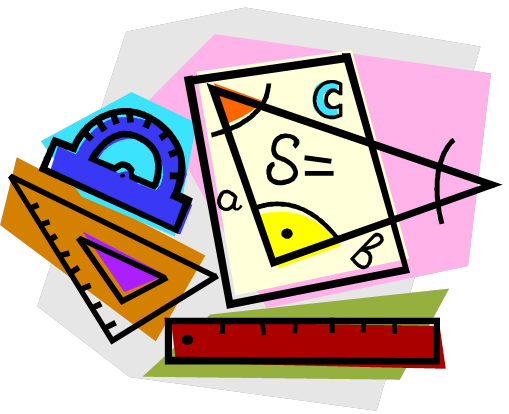
\includegraphics[width=4cm]{img-03/chap3.png}
}
{chap:trig}
 

\section{Raons trigonomètriques}
	\subsection{Raons trigonomètriques d'angle agut}

\begin{theorybox}
	
	Definim les raons trigonomètriques d'un angle agut d'un \textbf{triangle rectangle} com
	
	\begin{center}
		\textbf{sinus}: $\sin \alf = \dfrac{C.O.}{H}$, \textbf{cosinus}: $\cos \alf = \dfrac{C.C.}{H}$ i \textbf{tangent}: $\tg \alf = \dfrac{C.O.}{C.C.}$
	\end{center}
	
	essent $H$ la hipotenusa, $C.O.$ el catet oposat a l'angle i $C.C.$ el catet contigu. 
	
	També definim les raons recíproques com 
	
	\begin{center}
		\textbf{cosecant}:	$\cosec \alf = \dfrac{1}{\sin \alf}$, \textbf{secant}: $\sec \alf = \dfrac{1}{\cos \alf}$ i \textbf{cotangent}: $\cotg \alf = \dfrac{1}{\tg \alf}$.
	\end{center}
	
	
	\begin{minipage}{0.65\textwidth}
		\vspace{-0.75cm}	
		\video{122}{Raons d'un angle agut}
		
		\vspace{0.4cm}
		Representació de les raons trigonomètriques per un angle agut. Les raons no depenen de 
		la mida del triangle; només de l'angle.
	\end{minipage}
	\begin{minipage}{0.35\textwidth}
		
		\begin{center}
			\includegraphics*[width=0.8\textwidth]{img-03/chap-trig-grafraons.png}
		\end{center}
	\end{minipage}
\end{theorybox}

\begin{mylist}
	\exer
	A partir d'un triangle rectangle i aplicant el teorema de \emph{Pitàgores}, demostra la primera relació fonamental de la trigonometria $\sin^2 \alpha + \cos^2 \alpha = 1$.
	
	\answers{Si el triangle rectangle té hipotenusa $a$ i catets $b$ i $c$. Es compleix per trigonometria que $b=a\cos \alpha$ i $c=a\sin \alpha$. Si aplicam el teorema de Pitàgores a aquest triangle $a^2 = b^2 + c^2$, trobam que $a^2 = (a\cos \alpha)^2+ (a\sin \alpha)^2$. Finalment, simplificam dividint entre $a^2$  trobam $\sin^2 \alpha + \cos^2 \alpha = 1$.}
 	
	\exer
	Utilitzant les definicions de les raons trigonomètriques, demostra la
	segona relació fonamental $\tg \alpha = \dfrac{\sin \alpha}{\cos \alpha}$.
	\answers{$\dfrac{\sin \alpha}{\cos \alpha}=\dfrac{\frac{CO}{H}}{\frac{CC}{H}}=\dfrac{CO}{CC}=\tg \alpha$}
	
	\exer
	Utilitzant la definició de les raons, demostra les identitats:
	\begin{tasks}(2)
		\task $1+\tg^2 \alf = \sec^2 \alf$
		\task $1+\cotg^2 \alf = \cosec^2 \alf$
	\end{tasks}
	
	Comprova les anteriors relacions a partir dels angles de
	30${}^\circ$ i 60 ${}^\circ$.
	\answers{a) Parteix de $\sin^2 \alpha + \cos^2 \alpha = 1$ i divideix tot entre $\cos^2 \alpha$.\par b) Parteix de $\sin^2 \alpha + \cos^2 \alpha = 1$ i divideix tot entre $\sin^2 \alpha$}
	
	\exer
	Explica, a partir del vist en aquest apartat, perquè el sinus i el
	cosinus de 45${}^\circ$ són iguals, i perquè la tangent val
	la unitat.
	\answers{A 45 graus, resulta que CC=CO i per això $\sin 45 = \cos 45$.\par Com que la $\tg 45 = \dfrac{CO}{CC}=1$.}
\end{mylist}

\begin{theorybox}[Raons d'angles notables aguts]
	\videonw{124}{Trigonometria: Demostració de les raons dels angles notables 0, 30, 45, 60 i 90 graus}
	
	\begin{center}
		\renewcommand*{\arraystretch}{1.3}
		\begin{longtable}{|P{0.15\textwidth}|P{0.15\textwidth}|P{0.15\textwidth}|P{0.15\textwidth}|P{0.15\textwidth}|}
			\rowcolor{lightgray} Angle $\alpha$ (${}^\circ$) & Angle $\alpha$ (rad) & $\sin \alpha$ & $\cos \alpha$ & $\tg \alpha$ \\ \hline
			0 & 0 & 0 & 1 & 0 \\ \hline
			30 & $\frac{\pi}{6}$ & $\frac{1}{2}$  & $\frac{\sqrt{3}}{2}$  & $\frac{\sqrt{3}}{3}$ \\ \hline
			45 & $\frac{\pi}{4}$ & $\frac{\sqrt{2}}{2}$ & $\frac{\sqrt{2}}{2}$  & 1 \\ \hline
			60 & $\frac{\pi}{3}$ & $\frac{\sqrt{3}}{2}$  & $\frac{1}{2}$  &  $\sqrt{3}$ \\ \hline
			90 & $\frac{\pi}{2}$ & 1 & 0 & $--$ \\ \hline
		\end{longtable}
		
	\end{center}
	
\end{theorybox}

\subsection{Angles i raons trigonomètriques inverses}


\begin{theorybox} 
	\video{123}{}
	
	\textbf{Radiant}
	
	Un angle de 1 rad $\approx 57,3^\circ$. A la pràctica utilitzam el factor de conversió 
	\begin{equation*}
	2\pi\,\, \mathrm{rad} = 360^\circ.
	\end{equation*} 
\end{theorybox}

\begin{mylist}
	\exer Expressa en radiants els angles següents: 60${}^\circ$, 120${}^\circ$, 225${}^\circ$, 330${}^\circ$.
	\answers{$\frac{\pi}{3}$, $\frac{2}{3}\pi$, $\frac{5}{4}\pi$, $\frac{11}{6}\pi$}
	\begin{example}[*]
		\begin{equation*}
		60^\circ \cdot \frac{2 \pi \,\,\mathrm{rad}}{360^\circ} = \frac{60}{180}\pi = \frac{\pi}{3} \,\,\mathrm{rad}
		\end{equation*}
	\end{example}
	
	\exer 
	Expressa en graus sexagesimals: $\dfrac{\pi}{4}$, $\dfrac{2\pi}{3}$, $\dfrac{3\pi}{2}$ i $\dfrac{10\pi}{6}$ radiants.
	\answers{$45^\circ$, $120^\circ$, $270^\circ$, $300^\circ$}
	
	\exer 
	Quant sumen (en radiants) els angles d'un triangle? Quant mesura un
	angle recte en radiants?
	\answers{Els angles d'un triangle sumen $\pi$ radiants. Un angle recte són $\pi/2$ radiants.}
	
	\exer
	Per veure la utilitat dels radiants, suposem un mòbil que es mou en
	una circumferència de dos metres de radi amb una velocitat de 4 m/s.
	Calcula la seva velocitat en rad/s i en graus per segon. Quantes
	voltes dóna per minut?
	\answers{$\omega=v/R=2$ rad/s. En un minut \linebreak $2$ rad/s $\cdot 60 $s$ = 120 $ rad = 19.1 voltes}
	
	\exer
	Un mòbil ha recorregut un angle de 3 rad en una circumferència de radi 2 m. Quant
	espai ha recorregut? I si la circumferència tingués radi 0'5 m? \emph{Recorda}:  
	L'arc de circumferència $s$ és $s=\alpha\cdot R$ si l'angle $\alpha$ ve en radiants.
	\answers{6 m i 1.5 m}
	
\end{mylist}


\subsection{Raons trigonomètriques d'angles qualssevol}
\begin{theorybox}
	\video{125}{Raons trigonomètriques d'angles qualssevol}
	
	Signe de les raons trigonomètriques segons el quadrant:
	\begin{center}
		\includegraphics*[width=0.4\textwidth]{img-03/chap-trig-signesraons.png}
	\end{center}
\end{theorybox}

\begin{blueshaded}
	La calculadora té dos modes per manejar angles, \textbf{DEG} graus i \textbf{RAD} radiants. Per aquesta activitat assegura't que el tens en mode \textbf{DEG}.
	
	\begin{minipage}{0.6\textwidth}
		Les funcions trigonomètriques inverses de la calculadora donen només un dels possibles possibles de l'angle. Aquest angle es troba entre:
	\end{minipage}
	\begin{minipage}{0.4\textwidth}
		\begin{center}
			\begin{tabular}{c|c}
				$\arcsin x$ & $-90^\circ$ a $90^\circ$ \\ \hline
				$\arccos x$ & $0^\circ$ a $180^\circ$ \\ \hline
				$\arctg x$ & $-90^\circ$ a $90^\circ$ \\	
			\end{tabular}
		\end{center}
	\end{minipage}
	
	L'altre angle l'has d'obtenir raonant amb l'ajuda de la circumferència goniomètrica.
	
	\textbf{Quins angles tenen per sinus 0,5?}
	
	Una resposta l'obtenim de la calculadora \tecla{SHIFT} \tecla{sin} 0,5 \tecla{=} \pantalla{30}.
	
	L'altre angle es troba al segon quadrant, i l'obtenim fent $180^\circ-30^\circ=150^\circ$
	
	\textbf{Quins angles tenen per tangent -2?}
	
	Una resposta l'obtenim de la calculadora \tecla{SHIFT} \tecla{tan} -2 \tecla{=} \pantalla{-63.4349...}. Aquest angle es troba al quart quadrant i en
	realitat és l'angle $360-63,4349=296.5651$.
	
	L'altre angle s'ha de trobar al segon quadrant, on també la tangent és negativa. El trobam fent $180^\circ-63,3349^\circ=116,5651^\circ$
\end{blueshaded}
\begin{mylist}	
	\exer
	Copia en el teu quadern, i situa en el quadrant que correspongui i
	expressa en funció d'un angle agut les raons trigonomètriques dels
	següents angles:
	\begin{tabular}{|p{0.10\textwidth}|p{0.11\textwidth}|p{0.11\textwidth}|p{0.11\textwidth}|p{0.11\textwidth}|p{0.11\textwidth}|p{0.11\textwidth}|}
		\toprule
		Angle & Sinus & Cosinus & Tangent & Secant & Cosecant & Cotangent \\
		\midrule
		120$^\circ$ & & & & & & \\ \hline
		135$^\circ$ & & & & & & \\ \hline
		210$^\circ$ & & & & & & \\ \hline
		315$^\circ$ & & & & & & \\ \hline
		390$^\circ$ & & & & & & \\ \hline
		3000$^\circ$ & & & & & & \\ \hline
		$-150^\circ$ & & & & & & \\  
		\bottomrule
	\end{tabular}
\answers{ $\bullet$ \textbf{120 = 180--60} \par\par
	$\sin 120=\sin 60$\par$\cos 120=-\cos 60$\par$\tg 120=-\tg 60$\par\par
	$\bullet$ \textbf{135 = 180--45} \par\par
	$\sin 135=\sin 45$\par$\cos 135=-\cos 45$\par$\tg 135=-\tg 45$\par\par
	$\bullet$ \textbf{210 = 180+30} \par\par
	$\sin 210=-\sin 30$\par$\cos 210=-\cos 30$\par$\tg 210=\tg 30$\par\par
	$\bullet$ \textbf{315= 360--45} \par\par
	$\sin 315=-\sin 45$\par$\cos 315=\cos 45$\par$\tg 315=-\tg 45$\par\par
	$\bullet$ \textbf{390 = 30} \par\par
	$\sin 390=\sin 30$\par$\cos 390=\cos 30$\par$\tg 390=\tg 30$\par\par
	$\bullet$ \textbf{3000 = 120} \par\par
	$\sin 3000=\sin 120$\par$\cos 3000=\cos 120$\par$\tg 3000=\tg 120$\par\par
	$\bullet$ \textbf{--150 = 210} \par\par
	$\sin -150=\sin 210$\par$\cos -150=\cos 210$\par$\tg -150=\tg 210$\par\par
}
	
	\exer
	Utilitza la calculadora i l'après en aquest apartat per trobar tots
	els angles positius menors que 360${}^\circ$ el sinus dels quals
	és de 0'6.
	\answers{Una solució $\arcsin 0,6=36.87^\circ$ l'altre és $180-36.87 =143.13^\circ$}
	
	\exer
	Troba tots el angle compresos entre 0 i $360^\circ$ la tangent dels quals val 4.
	\answers{Una solució $\arctg 4=75.96^\circ$ l'altre és $180+75.96 =255.96^\circ$}
	
	\exer
	Troba tots el angle compresos entre 0 i $360^\circ$ el cosinus dels quals val 0'75.
	\answers{Una solució $\arccos 0.75=41.41^\circ$ l'altre és $360-41.41 =318.59^\circ$}
	
\end{mylist}	



\section{Resolució de triangles}

\subsection{Triangles rectangles}

\begin{theorybox}
	\begin{wrapfigure}{r}{4cm}
		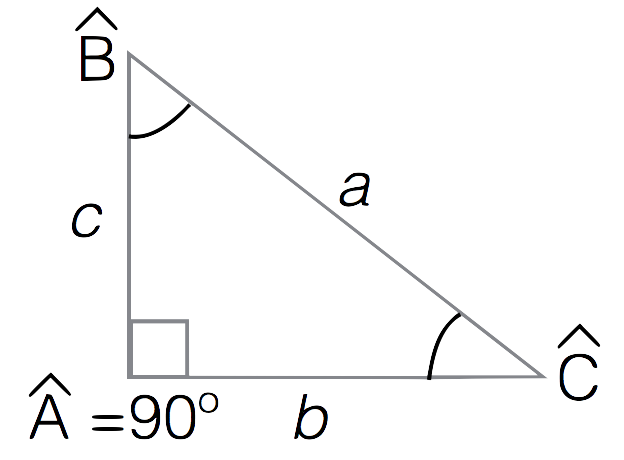
\includegraphics[width=4cm]{img-03/triangle-rectangle1}
	\end{wrapfigure}
	En un triangle rectangle, sempre utilitzarem el següent conveni per anomenar els costats i angles. L'angle recte és $\hat A=90^\circ$.
	
	Podrem utilitzar les següents relacions
	\begin{eqnarray*}
		\hat B=90-C, & a^2 = b^2 + c^2
	\end{eqnarray*}
	\begin{eqnarray*}
		b=a \cos \hat C, & c=a \sin \hat C, & \tg \hat C= \dfrac{c}{b}
	\end{eqnarray*}	
\end{theorybox}

\begin{resolt}[E]{Resol el triangle rectangle del qual sabem que \linebreak $\hat B=50^\circ$ i el catet $c=15$ cm.}
	
	\begin{wrapfigure}{r}{3.75cm}
		\vspace{-0.3cm}
		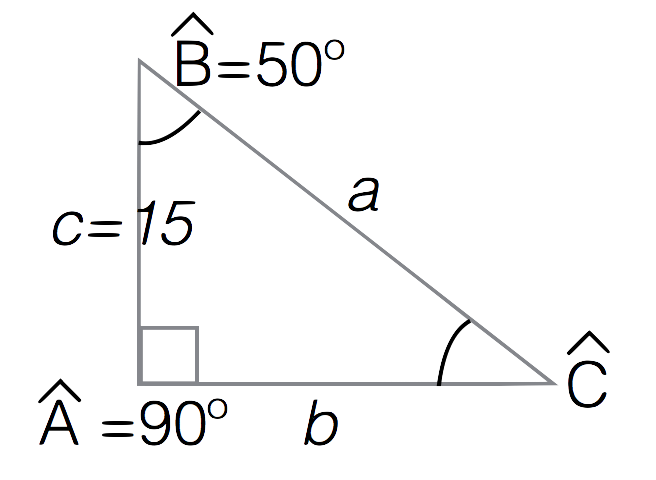
\includegraphics[width=3.5cm]{img-03/triangle-rectangle2}
	\end{wrapfigure}
	L'angle $\hat C$ s'obté de $\hat C=90-50 = 40^\circ$.
	
	Tot seguit, utilitzam la raó trigonomètrica \vspace{0.25cm}
	
	$\tg 40 = \dfrac{15}{b}$  $\rightarrow$ $b=\dfrac{15}{\tg 40}=17,87$.
	
	Del teorema de Pitàgores, $a^2 = b^2 +c^2$, \vspace{0.25cm}
	
	$a=\sqrt{15^2+17,87^2}=23,34$
	
\end{resolt}


\begin{mylist}
	
	\exer[1] Resol el triangle ABC (calcula els elements que falten), essent A l'angle recte
	\begin{tasks}(2)
		\task a=32 cm, B=57$^\circ$
		\task a=72 cm, C=23$^\circ$
		\task c=250 m, b=308 m
		\task c=35 m, C=32$^\circ$
	\end{tasks}
	\answers[cols=1]{[$\hat C=33$; $b=26,8$; $c=17,4$,  $\hat B=67$; $b=66,3$; $c=28,1$,  $\hat C=39$; $\hat B=51$; $a=396,7$,  $\hat B=58$; $b=56,01$; $a=66,05$]}
	
	\exer[1] Per arribar a una alçada de 3 m, recolçam una escala formant un angle de 60$^\circ$ amb el terra. Troba la longitud de l'escala i la distància des de la base fins a la paret.
	\answers{$a=3,46$; $b=1,73$}
	
	\exer[1] L'estatura d'una persona és 1,78 m i projecta al terra una ombra de 85 cm. Quin angle formen els rajos del sol amb l'horitzontal del terra?
	\answers{$\alpha=25,5^\circ$}
	
	\exer[1]
	Calcula els costats i els angles del triangle \emph{ABC}, rectangle en
	A, del que coneixem el catet \emph{AC} = 15cm i l'altura relativa a
	la hipotenusa \emph{AD} = 12cm.
	\answers{ $a=25$; $c=20$; $\hat B=36,87^\circ$; $\hat C=53,13^\circ$}
	
 
	\exer
	En un tram de carretera la inclinació és del 5 \% (puja 5 m en 100 m).
	Calcular l'angle que forma amb l'horitzontal la carretera. Sabem que
	hem pujat 100 m, quant hem caminat per la carretera?
	\answers{$\tg \alpha = 5/100$, $\alpha = 2.86^\circ$. $s=\frac{h}{\tg \alpha} = \frac{ 100}{\tg 2.86}=2000$ m. Hem caminat 2 km.}
	
	
	\exer \spicy[1] Una estàtua de 2,5 m d'altura està col·locada sobre una peanya. Des d'un punt del terra es veu la peanya amb un angle de 15$^\circ$ i l'estàtua, sobre un angle de 40$^\circ$. Quina és l'altura de la peanya?
	\answers{$x=\dfrac{2.5}{\tg 40 - \tg 15}=4.377$ m;  $y=x \tg 15 = 1.173$ m}
	
\end{mylist}

\subsection{Teorema del sinus}

\begin{theorybox}
	\video{127}{Trigonometria: Teorema del sinus}
	
	Sempre utilitzarem el següent conveni per anomenar els costats i angles.
	
	\begin{wrapfigure}{R}{4.5cm}
		\centering
		\vspace{-1.5cm}
		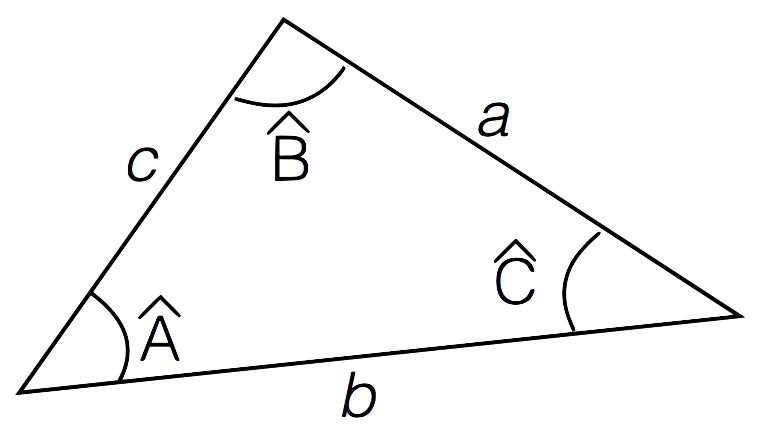
\includegraphics[width=4.5cm]{img-03/triangle-qualsevol1}
	\end{wrapfigure}
	
	D'una banda sabem que els angles compleixen $\hat A+\hat B+\hat C=180^\circ$. El teorema del sinus diu que 
	\begin{eqnarray*}
		\frac{a}{\sin \hat A}=\frac{b}{\sin \hat B}=\frac{c}{\sin \hat C}=2R
	\end{eqnarray*}
	on $R$ és el radi de la circumferència circumscrita en el triangle.
	
	De vegades, a l'aplicar el teorema del sinus, poden aparèixer dues solucions. 
	\vspace{0.7cm}
	
\end{theorybox}

\begin{resolt}[E]{En un triangle coneixem dos dels seus angles i un costat: A=55${}^\circ$, B=98${}^\circ$, a=7,5 cm. Resol el triangle.
		\begin{center}
			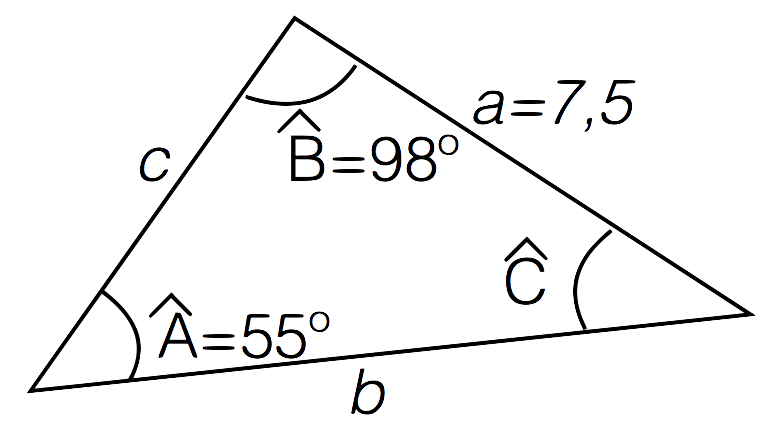
\includegraphics[width=4cm]{img-03/triangle-qualsevol2}
		\end{center}
}
	
	
	
	L'angle $\hat C=180 -(55+98)=27^\circ$
	
	Amb el teorema del sinus trobam els costats que falten
	\begin{eqnarray*}
		\frac{b}{\sin 98}= \frac{7,5}{\sin 55} \,\, \rightarrow \,\,  b=\frac{7,5 \sin 98}{\sin 55}=9,1 \,\mathrm{cm}\\
		\frac{c}{\sin 27}= \frac{7,5}{\sin 55} \,\, \rightarrow \,\,  c=\frac{7,5 \sin 27}{\sin 55}=4,2 \,\mathrm{cm}
	\end{eqnarray*}
	
	
\end{resolt}
\vspace{0.5cm}


\begin{mylist} 
	\exer
	Un triangle té dos angles que valen 40 i 60 graus respectivament. El
	costat entre ells és de 8 cm. Calcula tots els seus angles i costats.
	\answers{Costats:
		a = 5.22163 m
		b = 7.03508 m
		c = 8 m \par
		Angles:
		A = 40 
		B = 60 
		C = 80}
	
	\exer
	En un triangle \emph{ABC}, els costats \emph{AB} \emph{i AC} mesuren 3
	i 2 cm respectivament. L'angle corresponent al vèrtex \emph{B} mesura
	30 graus. Resol el triangle.
	\begin{tasks}
		\task Utilitza el teorema del sinus per calcular l'altre angle. Hi ha dues
		solucions perquè hi ha dos angles amb el mateix sinus. Calcula els dos.
		%
		\task Les dues solucions es deuen al fet que existeixen dos triangles, series
		capaç de dibuixar-los?
	\end{tasks}
	\answers{Té dues solucions:\par
	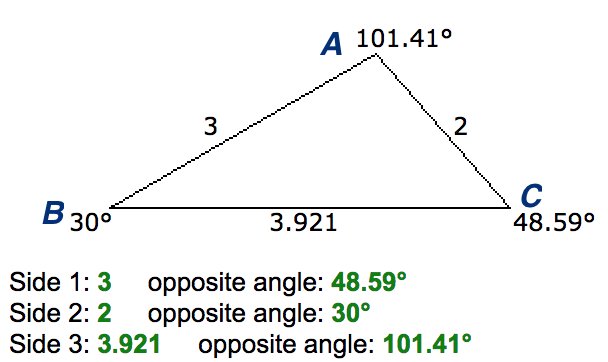
\includegraphics[width=0.4\textwidth]{img-sol/t3-21a}
	\par
	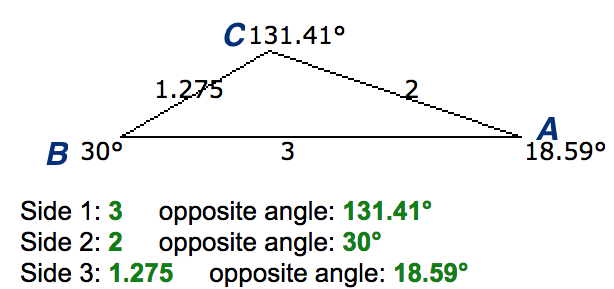
\includegraphics[width=0.4\textwidth]{img-sol/t3-21b}}
	
	
	\exer
	En un triangle coneixem dos dels seus angles i un costat: \emph{A=}55${}^\circ$, \emph{B}=98${}^\circ$, \emph{a=}7'5 cm. Resol-ho.
	\answers{Solució única:\par
		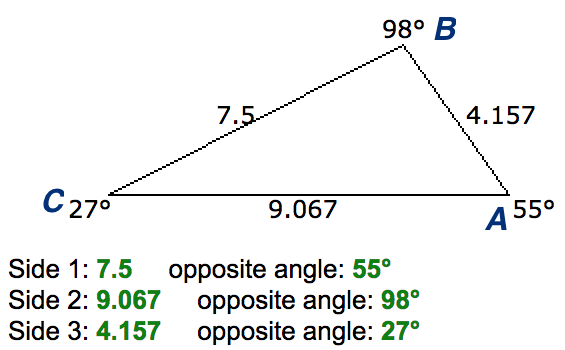
\includegraphics[width=0.4\textwidth]{img-sol/t3-22}}
		
	\exer El radi de la circumferència circumscrita al triangle ABC mesura $2\sqrt{2}$ i dos dels seus angles fan 60${}^\circ$ i 45${}^\circ$. Resol el triangle i troba'n l'àrea.
	

\answers{En primer lloc trobam dos costats a partir del radi: $a=4\sqrt{2}\sin 60=2\sqrt{6}$ i $b=4\sqrt{2} \sin 45 = 4$.\par 	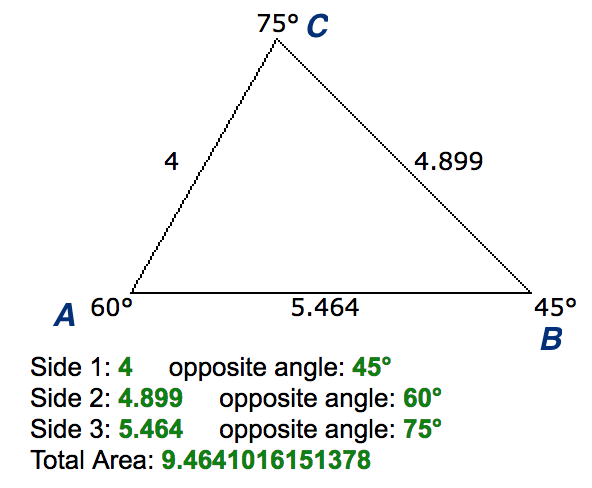
\includegraphics[width=0.4\textwidth]{img-sol/t3-23}}
	
	
	\exer
	Un globus està en la vertical entre dos observadors separats per 40 m.
	El primer ho veu amb un angle de 30 graus i el segon amb un angle de
	50 graus, a quina altura està el globus?
	
	\answers{En primer lloc resolem el triangle:\par 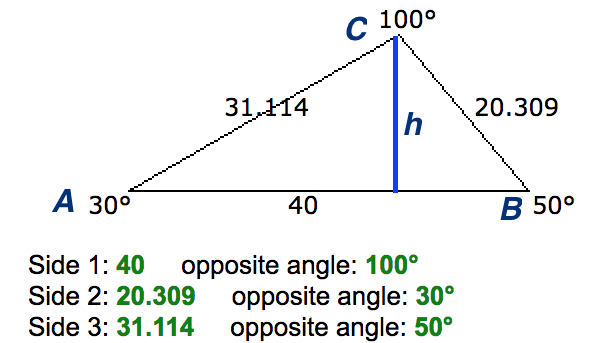
\includegraphics[width=0.4\textwidth]{img-sol/t3-24}\par
	Després calculam l'altura del triangle $h=31.1\sin 30=20.31\sin 50=15.6$ m}
	
	
	
	\exer
	Una antena de radi està subjecta al terra amb dos cables, que formen
	amb l'antena angles de 36${}^\circ$ i 48${}^\circ$. Els punts de subjecció dels cables	estan alineats amb el peu de l'antena i disten entre sí 98 metres.
	Calcula l'altura de l'antena.
	
	\answers{En primer lloc resolem el triangle:\par 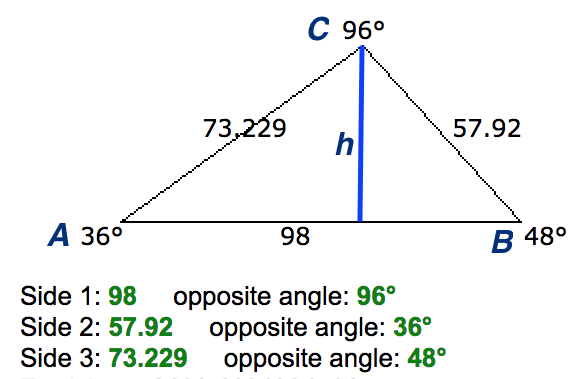
\includegraphics[width=0.4\textwidth]{img-sol/t3-25}\par
		Després calculam l'altura del triangle $h=73.23\sin 36=57.92\sin 48=43.04$ m}
	
	\exer
	Des d'un cert punt del terra es veu un arbre sota un angle de 42${}^\circ$. Baix
	quin angle es veu col·locant-se al doble de distància?
	\answers{La tangent de l'angle es redueix a la meitat: $\tg \alpha' = \frac{1}{2}\tg \alpha=\frac{1}{2}\tg 42=0.4502$, el nou angle és $\alpha'=\arctg 0.4502=24.24^\circ$. Evidentment no és la meitat de 42${}^\circ$.}
	
	\exer
	Dos amics estan en una platja a 150 m de distància i en el mateix
	plà vertical que un estel que es troba volant entre tots dos. En un
	moment donat, un el veu amb un angle d'elevació de 50${}^\circ$ i l'altre amb
	un angle de 38$^\circ$. Quina distància hi ha des de cadascun d'ells a
	l'estel? A quina altura vola l'estel?
	\answers{En primer lloc resolem el triangle:\par 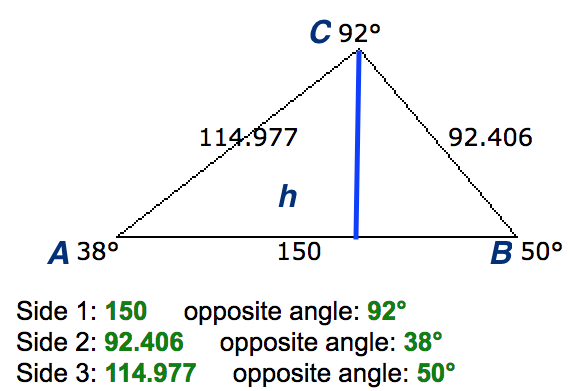
\includegraphics[width=0.4\textwidth]{img-sol/t3-27}\par
		Les distàncies de cadascú a l'estel són 115 m i 92.4 m. Després l'altura del triangle $h=114.98\sin 38=92.406\sin 50=70.79$ m}
	
	\exer
	Un globus aerostàtic es troba subjecte al terra mitjançant dos cables
	d'acer, en dos punts que disten 70 metres. El cable més curt mesura 90
	metres i l'angle que forma l'altre cable amb el terra és de 42${}^\circ$.
	Calcula:
	
	\begin{tasks}	 
		\task
		La mesura de l'altre cable.
		\task
		La distància del globus al terra.
	\end{tasks}

\answers{L'angle del triangle és $180-42=138$. En primer lloc resolem el triangle:\par 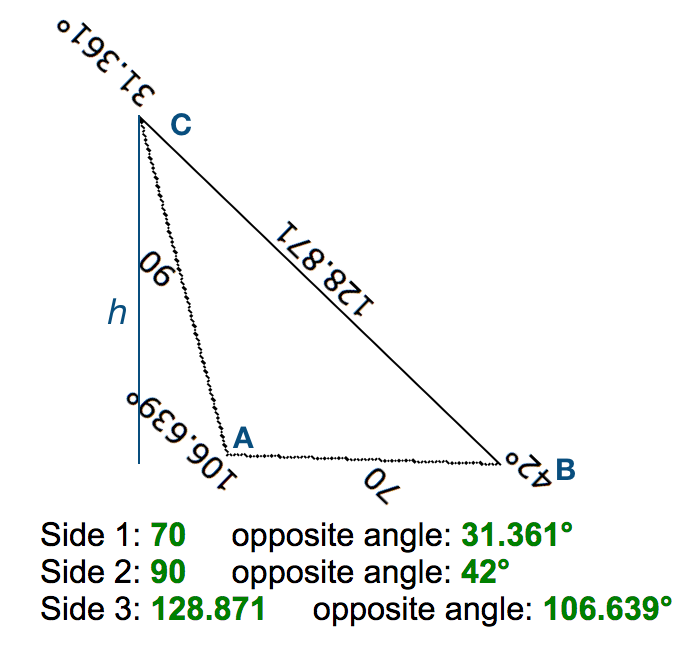
\includegraphics[width=0.4\textwidth]{img-sol/t3-28}\par
	L'altre cable mesura 128.87 m. La distància del globus al terra $h=128.87\sin 42=86.23$ m}
	
\end{mylist}

\subsection{Teorema del cosinus}

\begin{theorybox}
	\video{129}{Trigonometria: Teorema del cosinus}
	
	El teorema del cosinus s'aplica quan no tenim cap angle o quan tenim dos costats i l'angle que formen.
	El teorema es pot formular en tres versions diferents:
	\begin{eqnarray*}
		a^2 = b^2 + c^2 - 2  b \cdot c \cdot \cos\hat A \\
		b^2 = a^2 + c^2 - 2 a \cdot c\cdot \cos \hat B \\
		c^2 = a^2 + b^2 - 2 a \cdot b\cdot \cos \hat C 
	\end{eqnarray*}
	
	
\end{theorybox}


\begin{resolt}[E]{ En un triangle coneixem dos costats i l'angle comprès entre ells $\hat A$=35${}^\circ$, $b$=20 cm, $c$=14 cm. Resol-ho.}
	Aplicam el teorema del cosinus per trobar el costat oposat a l'angle A que ens donen. $a^2 = 20^2 + 14^2 - 2 \cdot 20 \cdot 14 \cos 35^\circ$.
	D'aquí aïllam el costat $a=11,72$ cm.
	
	Tornam a aplicar el teorema del cosinus ara pel costat $b$.
	
	$20^2 = 11,72^2 + 14^2 - 2 \cdot 11,72 \cdot 14 \cos \hat B$. D'aquesta fórmula cal aïllar el $\cos \hat B$,
	
	\begin{equation*}
	\cos \hat B = \dfrac{20^2 - 11,72^2 - 14^2}{-2 \cdot 11,72 \cdot 14}=-0,203
	\end{equation*}
	
	L'angle $\hat B=\arccos -0,203 = 101,7^\circ$, i finalment l'angle 
	
	 $\hat C=180-35-101,7=43,28^\circ$.
\end{resolt}

\begin{resolt}{Si els braços d'un compàs fan 12 cm de llarg i formen un angle de 60${}^\circ$, calcula el radi de la circumferència que podem traçar amb el compàs.}
	Aplicam el teorema el cosinus
	\begin{equation*}
	a^2 = 12^2 + 12^2 - 2 \cdot 12 \cdot 12 \cos 60^\circ
	\end{equation*}
	D'aquí s'obté que el costat oposat a l'angle de 60${}^\circ$ és de $a=12$, que correspon al radi
	de la circumferència que podem dibuixar. Es tracta d'un triangle isòsceles.
\end{resolt}

\begin{mylist}
	
	
	\exer
	Troba els angles d'un triangle del que es coneixen els tres costats:
	\emph{a=} 37 cm, \emph{b} = 42 cm, \emph{c} = 68 cm.
	
	\answers{$\hat A=28.52^\circ$, $\hat B=32.82^\circ$, $\hat C=118.66^\circ$}
	
	\exer
	Dibuixa un triangle amb b=5, c = 8 i l'angle entre ells de 30${}^\circ$ (usa
	una regla i un transportador). Calcula l'altre costat amb el teorema
	del cosinus i comprova que coincideix amb el resultat mesurat. No et
	sortirà exactament per l'arrodoniment i l'error de mesurament però
	hauria de ser molt similar.
	\answers{Triangle:\par 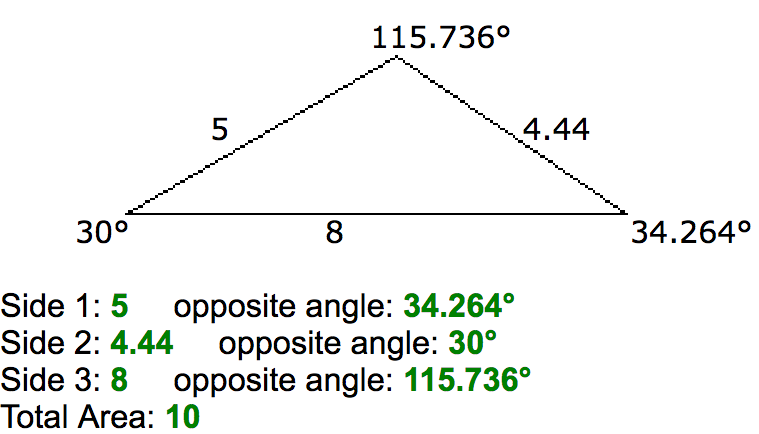
\includegraphics[width=0.4\textwidth]{img-sol/t3-30}}
	
	\exer
	Un triangle té de costats 3, 5 i 7. Calcula els seus angles.
		
	\answers{$\hat A=21.79^\circ$, $\hat B=38.21^\circ$, $\hat C=120^\circ$}
	
	
	\exer
	En un triangle \emph{ABC}, els costats \emph{AB} i\emph{AC} mesuren 3
	i 2 cm respectivament. L'angle corresponent al vèrtex \emph{B} mesura
	30 graus.
	
	a) Utilitza el teorema del cosinus per calcular l'altre costat.
	Obtindràs dues solucions.
	
	b) Les dues solucions es deuen al fet que hi ha dos triangles series
	capaç de dibuixar-los?
	
	\answers{Solució 1:\par
	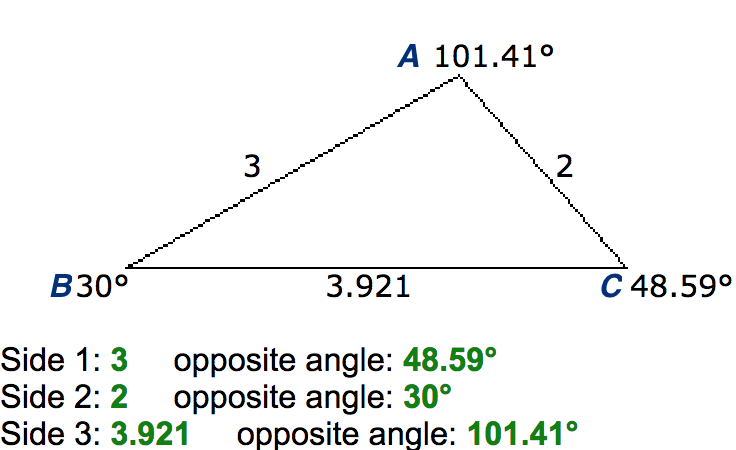
\includegraphics[width=0.4\textwidth]{img-sol/t3-32a}
	\par Solució 2:\par
	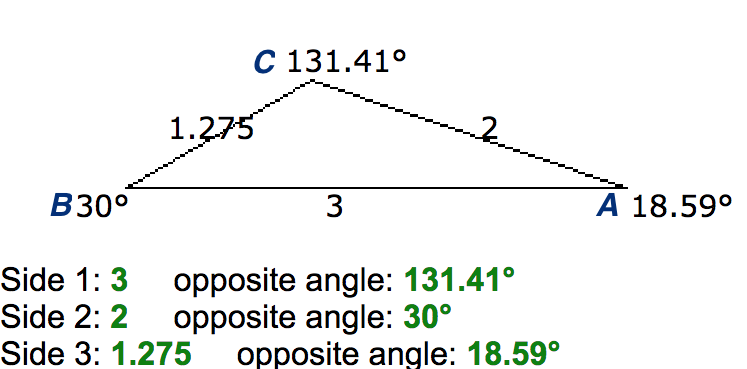
\includegraphics[width=0.4\textwidth]{img-sol/t3-32b}
}
	
	\exer
	Calcula  l'àrea d'un heptàgon regular inscrit en una circumferència de
	35 cm de perímetre.
	\answers{El radi de la circumferència $R=L/2\pi=5.57$ cm. El costat de l'heptàgon és $c=4.83$ cm  i l'apotema $a_p=5.02$  i l'àrea $A=84.9$ cm$^2$.\par 	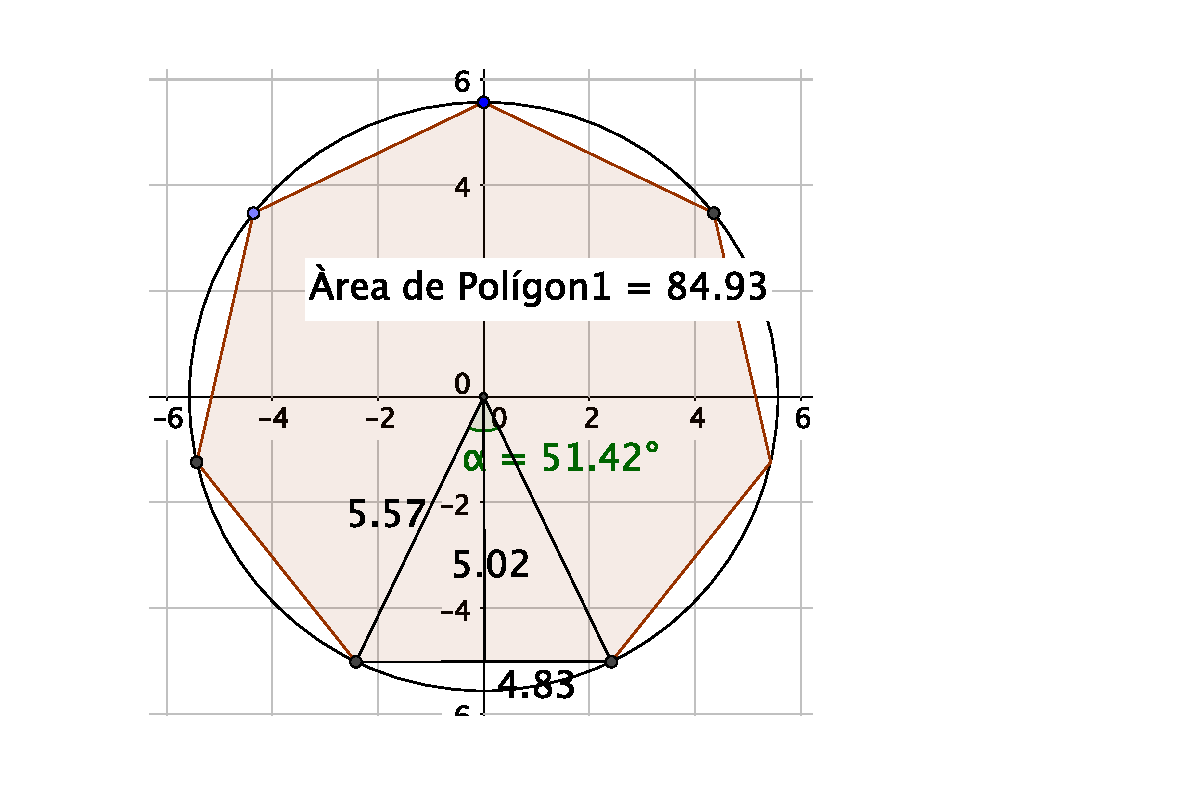
\includegraphics[width=0.3\textwidth]{img-sol/t3-33}}  
	
	\exer
	Dos vaixells parteixen d'un port amb rumbs diferents que formen un
	angle de 127${}^\circ$. El primer surt a les 10 h del matí amb una velocitat de
	17 nusos, i el segon surt a les 11 h 30 min, amb una velocitat de 26
	nusos. Si l'abast dels seus equips de radi és de 150 km. Podran
	posar-se en contacte a les 3 de la tarda? (nus=milla/hora; milla=1850
	m).
		\answers{Les distàncies en km recorregudes per cada vaixell són: $15\cdot 5 \, h \cdot 1.85=157.25$ km i  $26\cdot 3.5 \,h \cdot 1.85=168.35$ km. A les 15:00 es troben separats per 291.43 km que és superior a l'abast de le radi.\par 	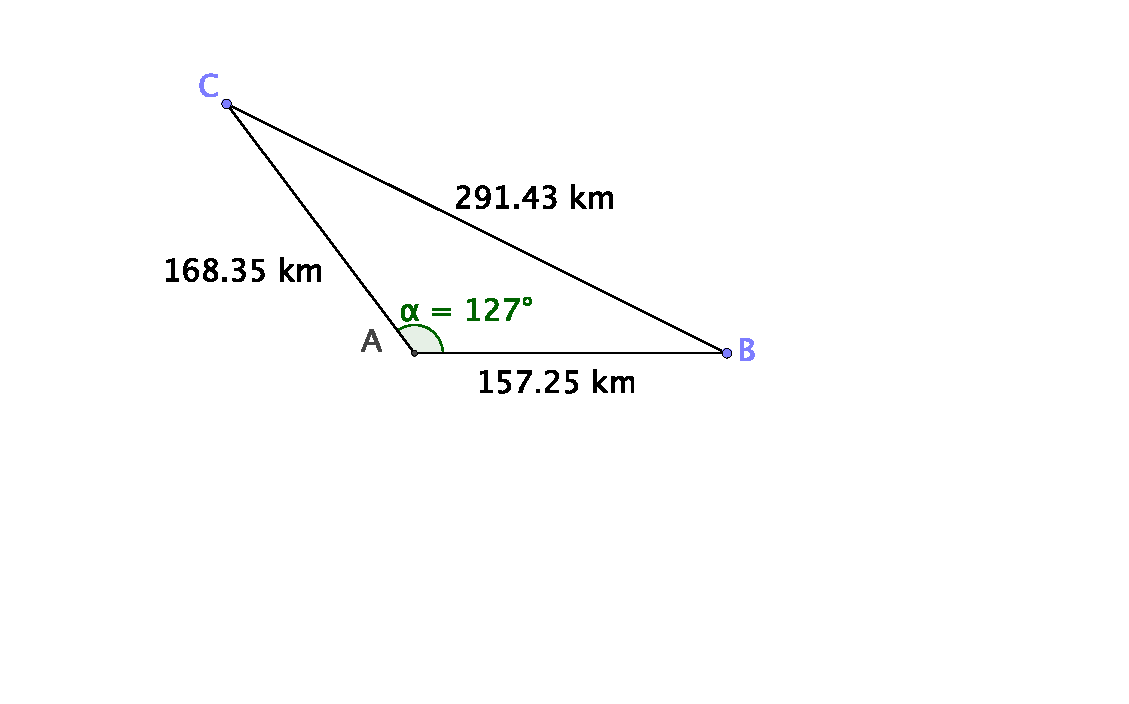
\includegraphics[width=0.4\textwidth]{img-sol/t3-34}}  
	
\end{mylist}

\subsection{Resolució de triangles en general}
\begin{mylist}
	
	
   	\vspace{-3cm}
\exer \begin{minipage}[t]{0.4\textwidth}
	Resol els següents triangles:  \vspace{0.2cm}
	\begin{tasks}
		\task B=30${}^\circ$, \emph{a}=5 cm, \emph{b} = 6 cm \vspace{0.2cm}
		\task A=45${}^\circ$, C=60${}^\circ$, \emph{b} = 20 m \vspace{0.2cm}
		\task C = 45${}^\circ$ , \emph{b} =10 m, \emph{c} = 6 m;  \vspace{0.2cm}
		\task \emph{a} = 5 cm, \emph{b} = 4 cm, \emph{c} = 4 cm \vspace{0.2cm}
		\task A=45${}^\circ$, \emph{b} = 50 m, \emph{a}=40 m
	\end{tasks}
\end{minipage}
\begin{minipage}{0.45\textwidth}
	
	\vspace{3cm}
	
	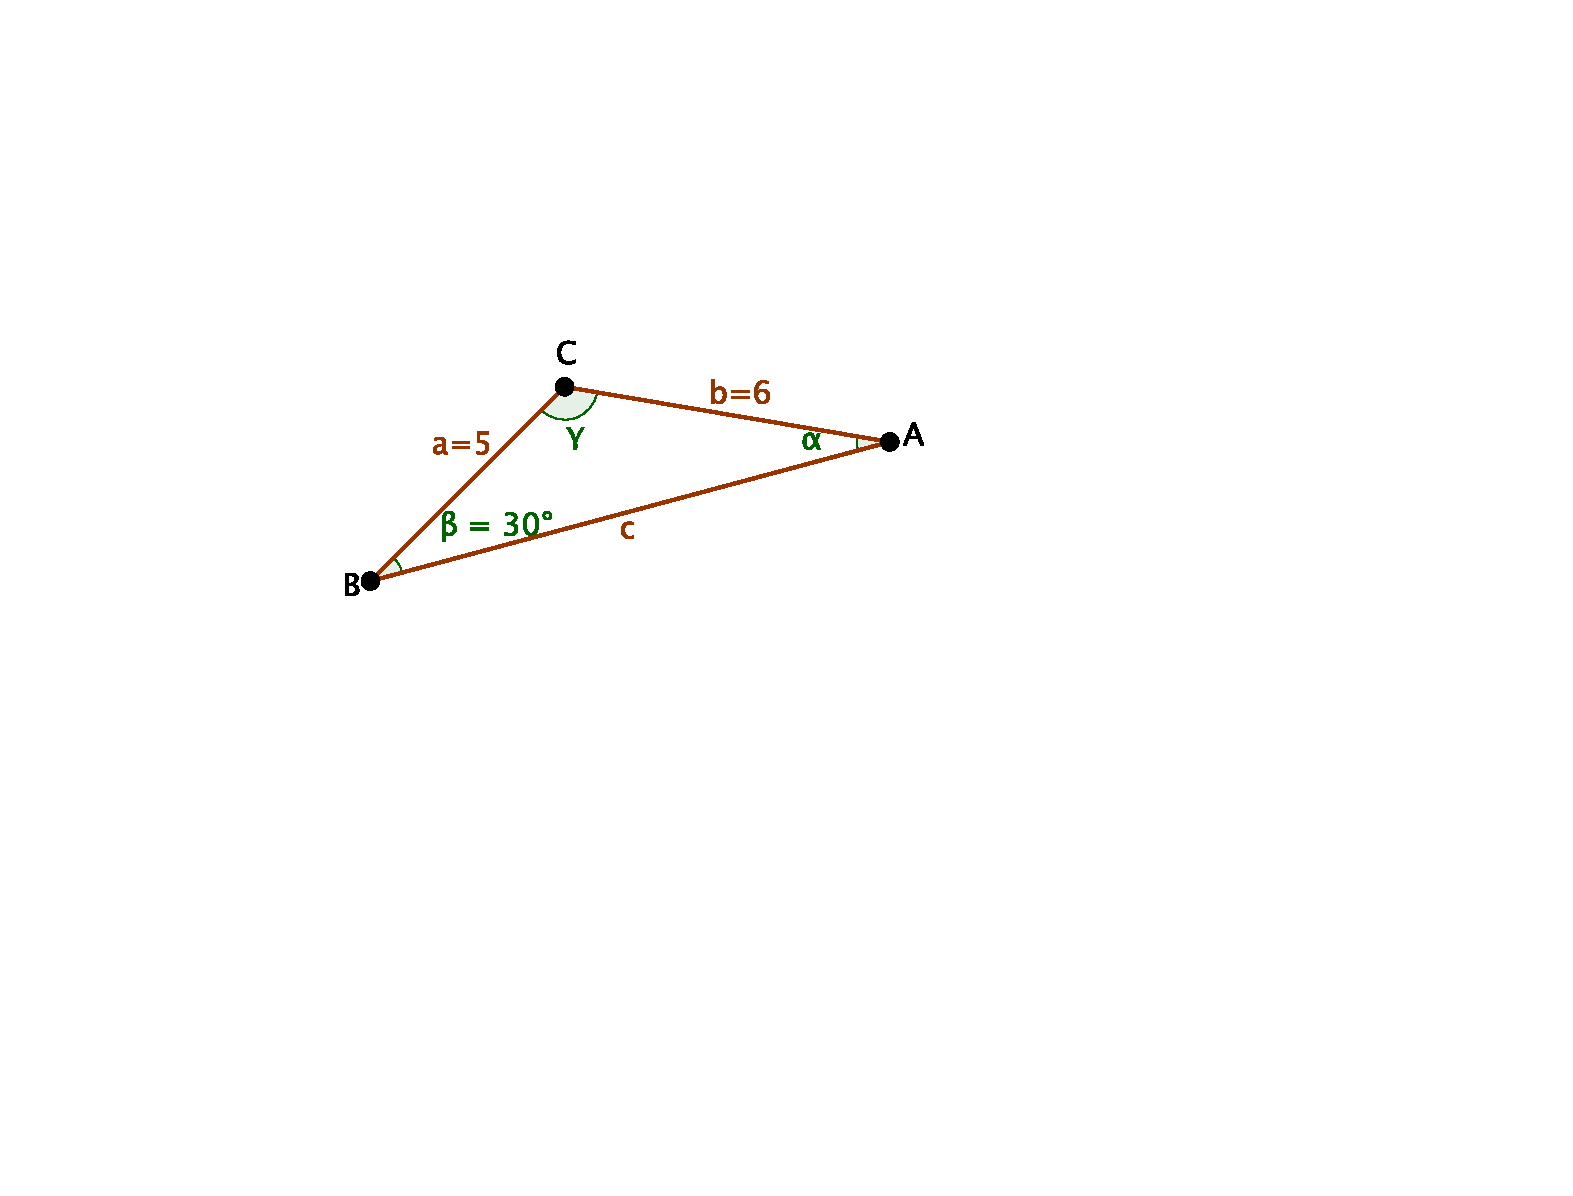
\includegraphics[width=0.9\textwidth]{img-03/trig-sample-triangle}
	
	{\footnotesize a) Representa els triangles deixant clares les dades i les incògnites.}
\end{minipage}
	\answers[cols=1]{[
 $A=24.52$; $C=125.38$; $c=9.78$,
$B=75$; $a=14.64$; $c=17.93$,
 No existeix cap triangle,
$A=77.36$; $B=C=51.32$,
Solució 1: $B=62.1$; $C=72.9$; $c=54.1$. 
Solució 2: $B=117.9$; $C=17.1$; $c=16.64$.]}x
	
	\exer
	Calcula l'àrea i el perímetre d'un pentàgon regular inscrit en una
	circumferència de radi 3 cm.
	
	\answers{El costat del polígon és $c=3.53$ cm  i l'apotema $a_p=2,43$  i l'àrea $A=21.4$ cm$^2$.\par 	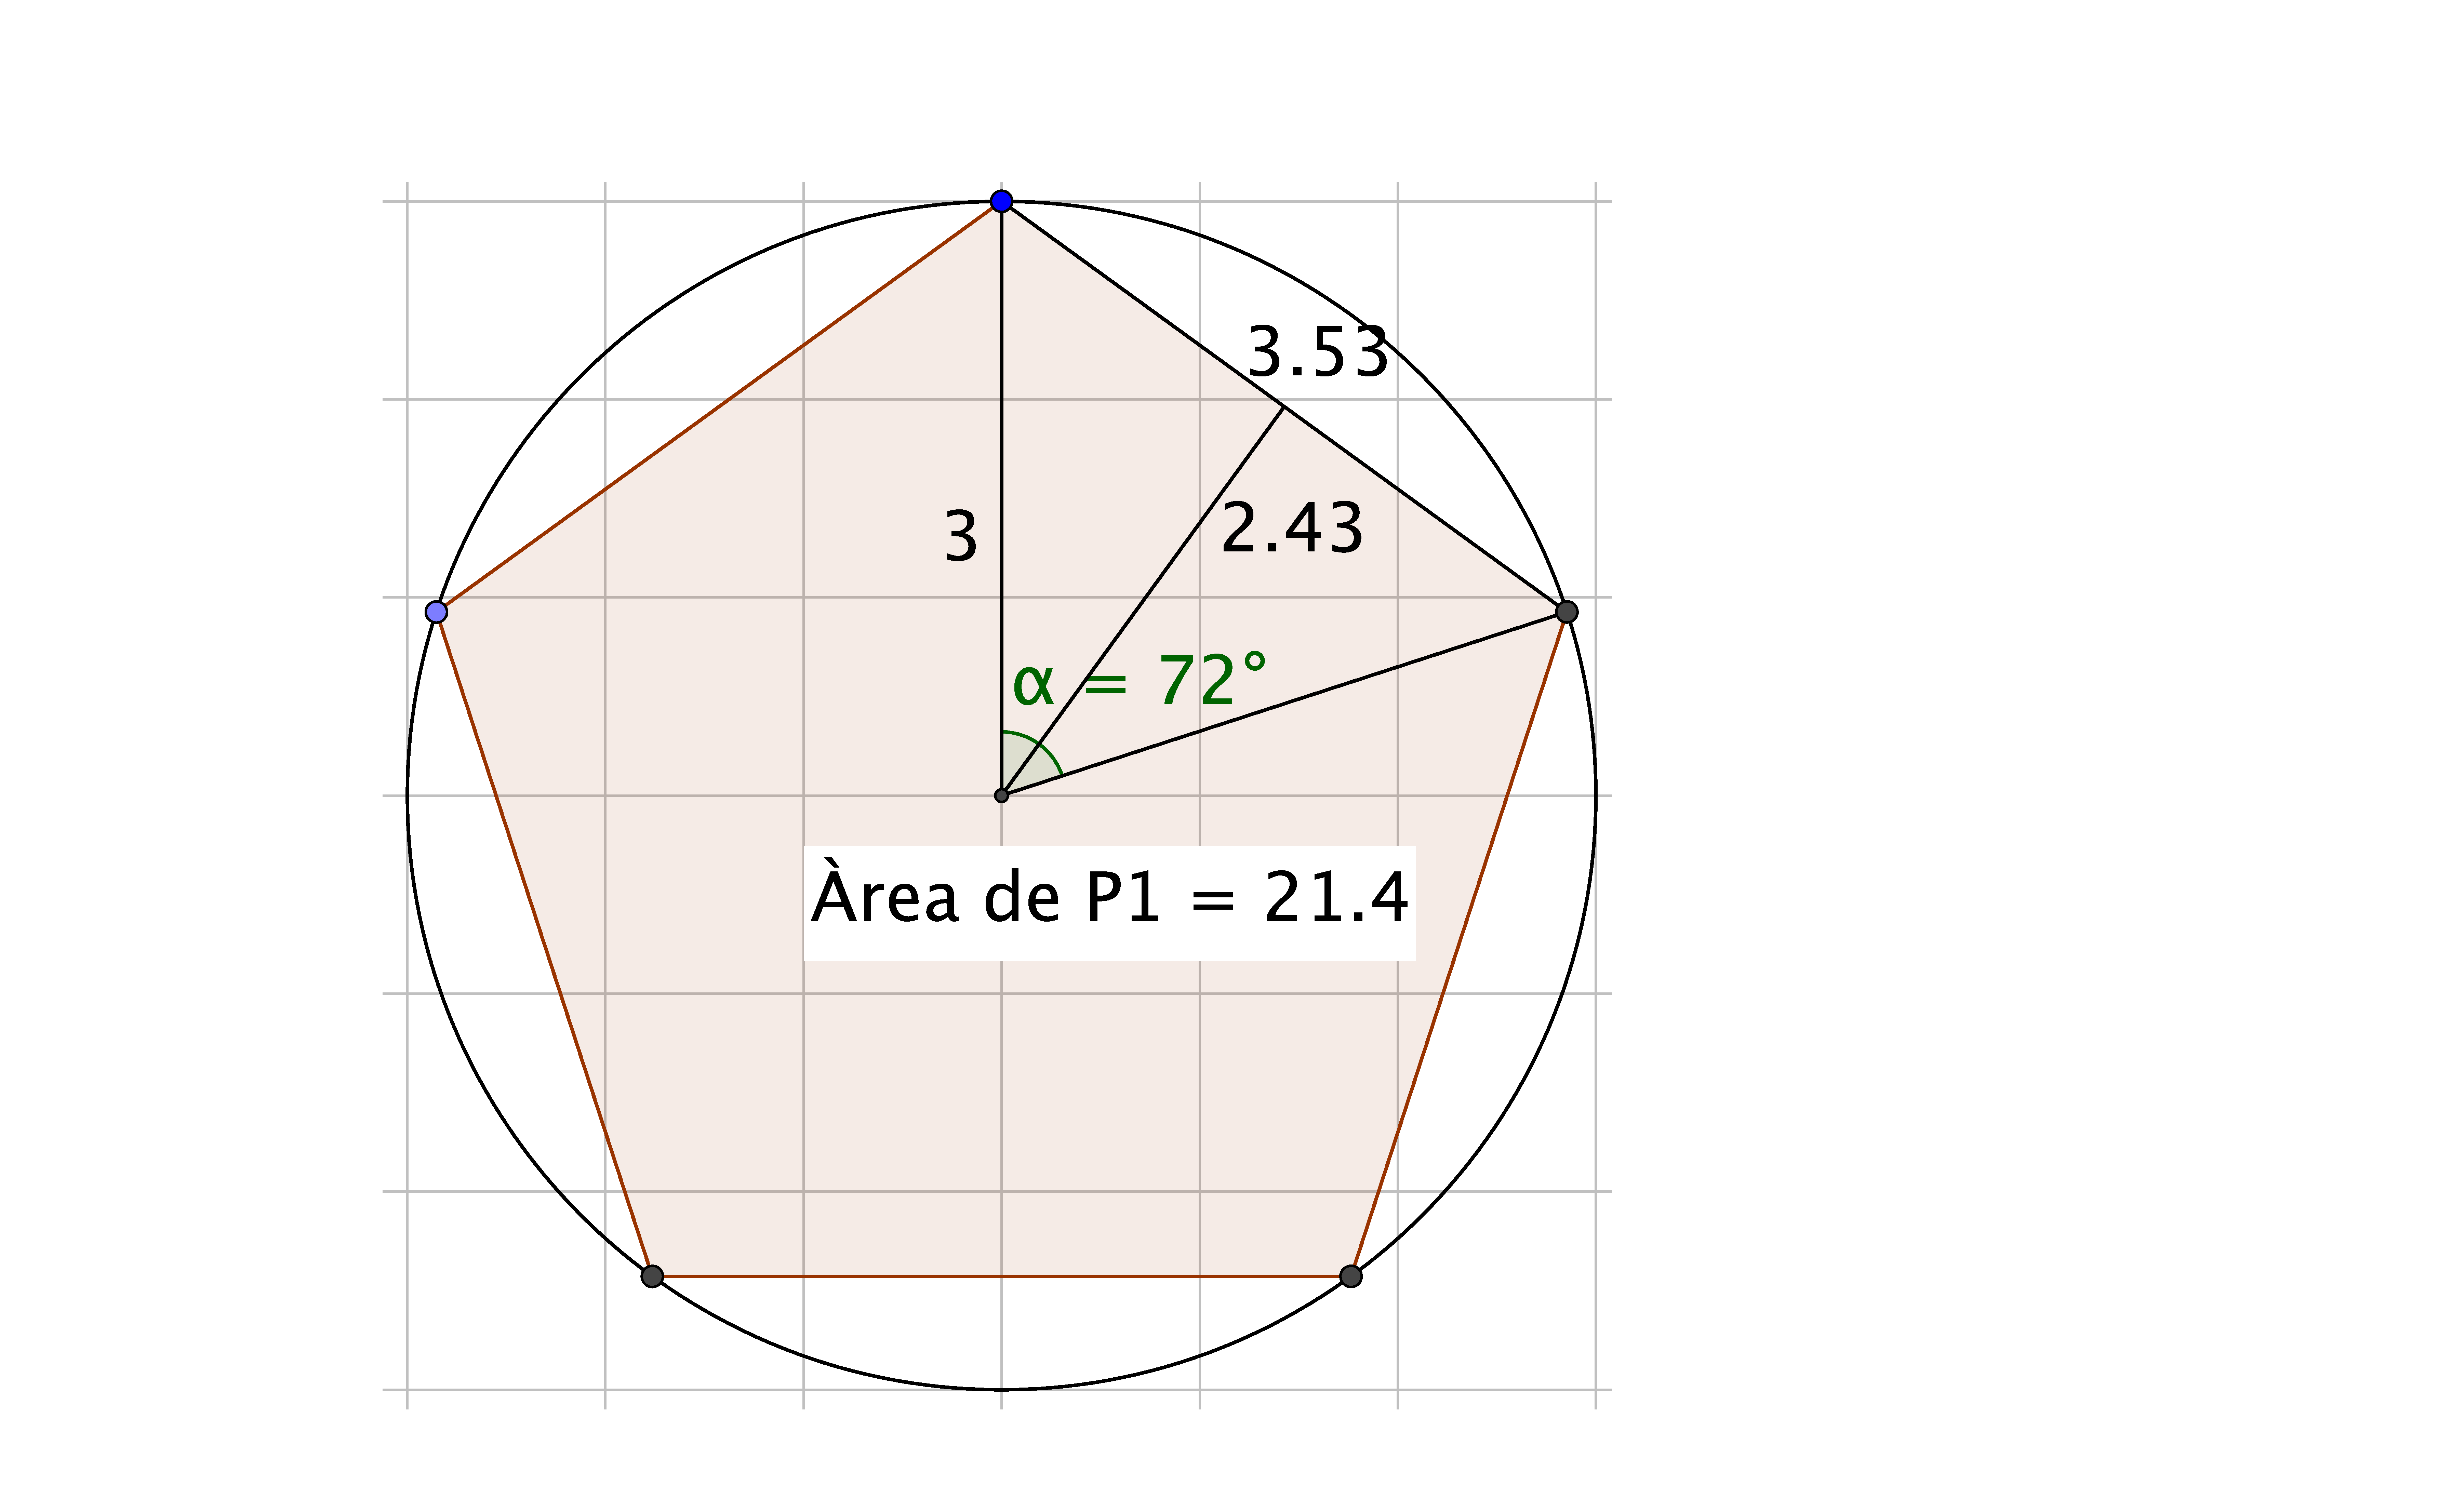
\includegraphics[width=0.3\textwidth]{img-sol/t3-36}}
	
	\pagebreak
	
	\exer
	Des d'un far \emph{F} es veu un vaixell A amb angle de 43${}^\circ$ amb la
	costa, i el vaixell B amb 21${}^\circ$. El vaixell \emph{B} està a 3 km de la
	costa i el A a 5 km. Calcula distància entre els vaixells.
	\begin{center}
		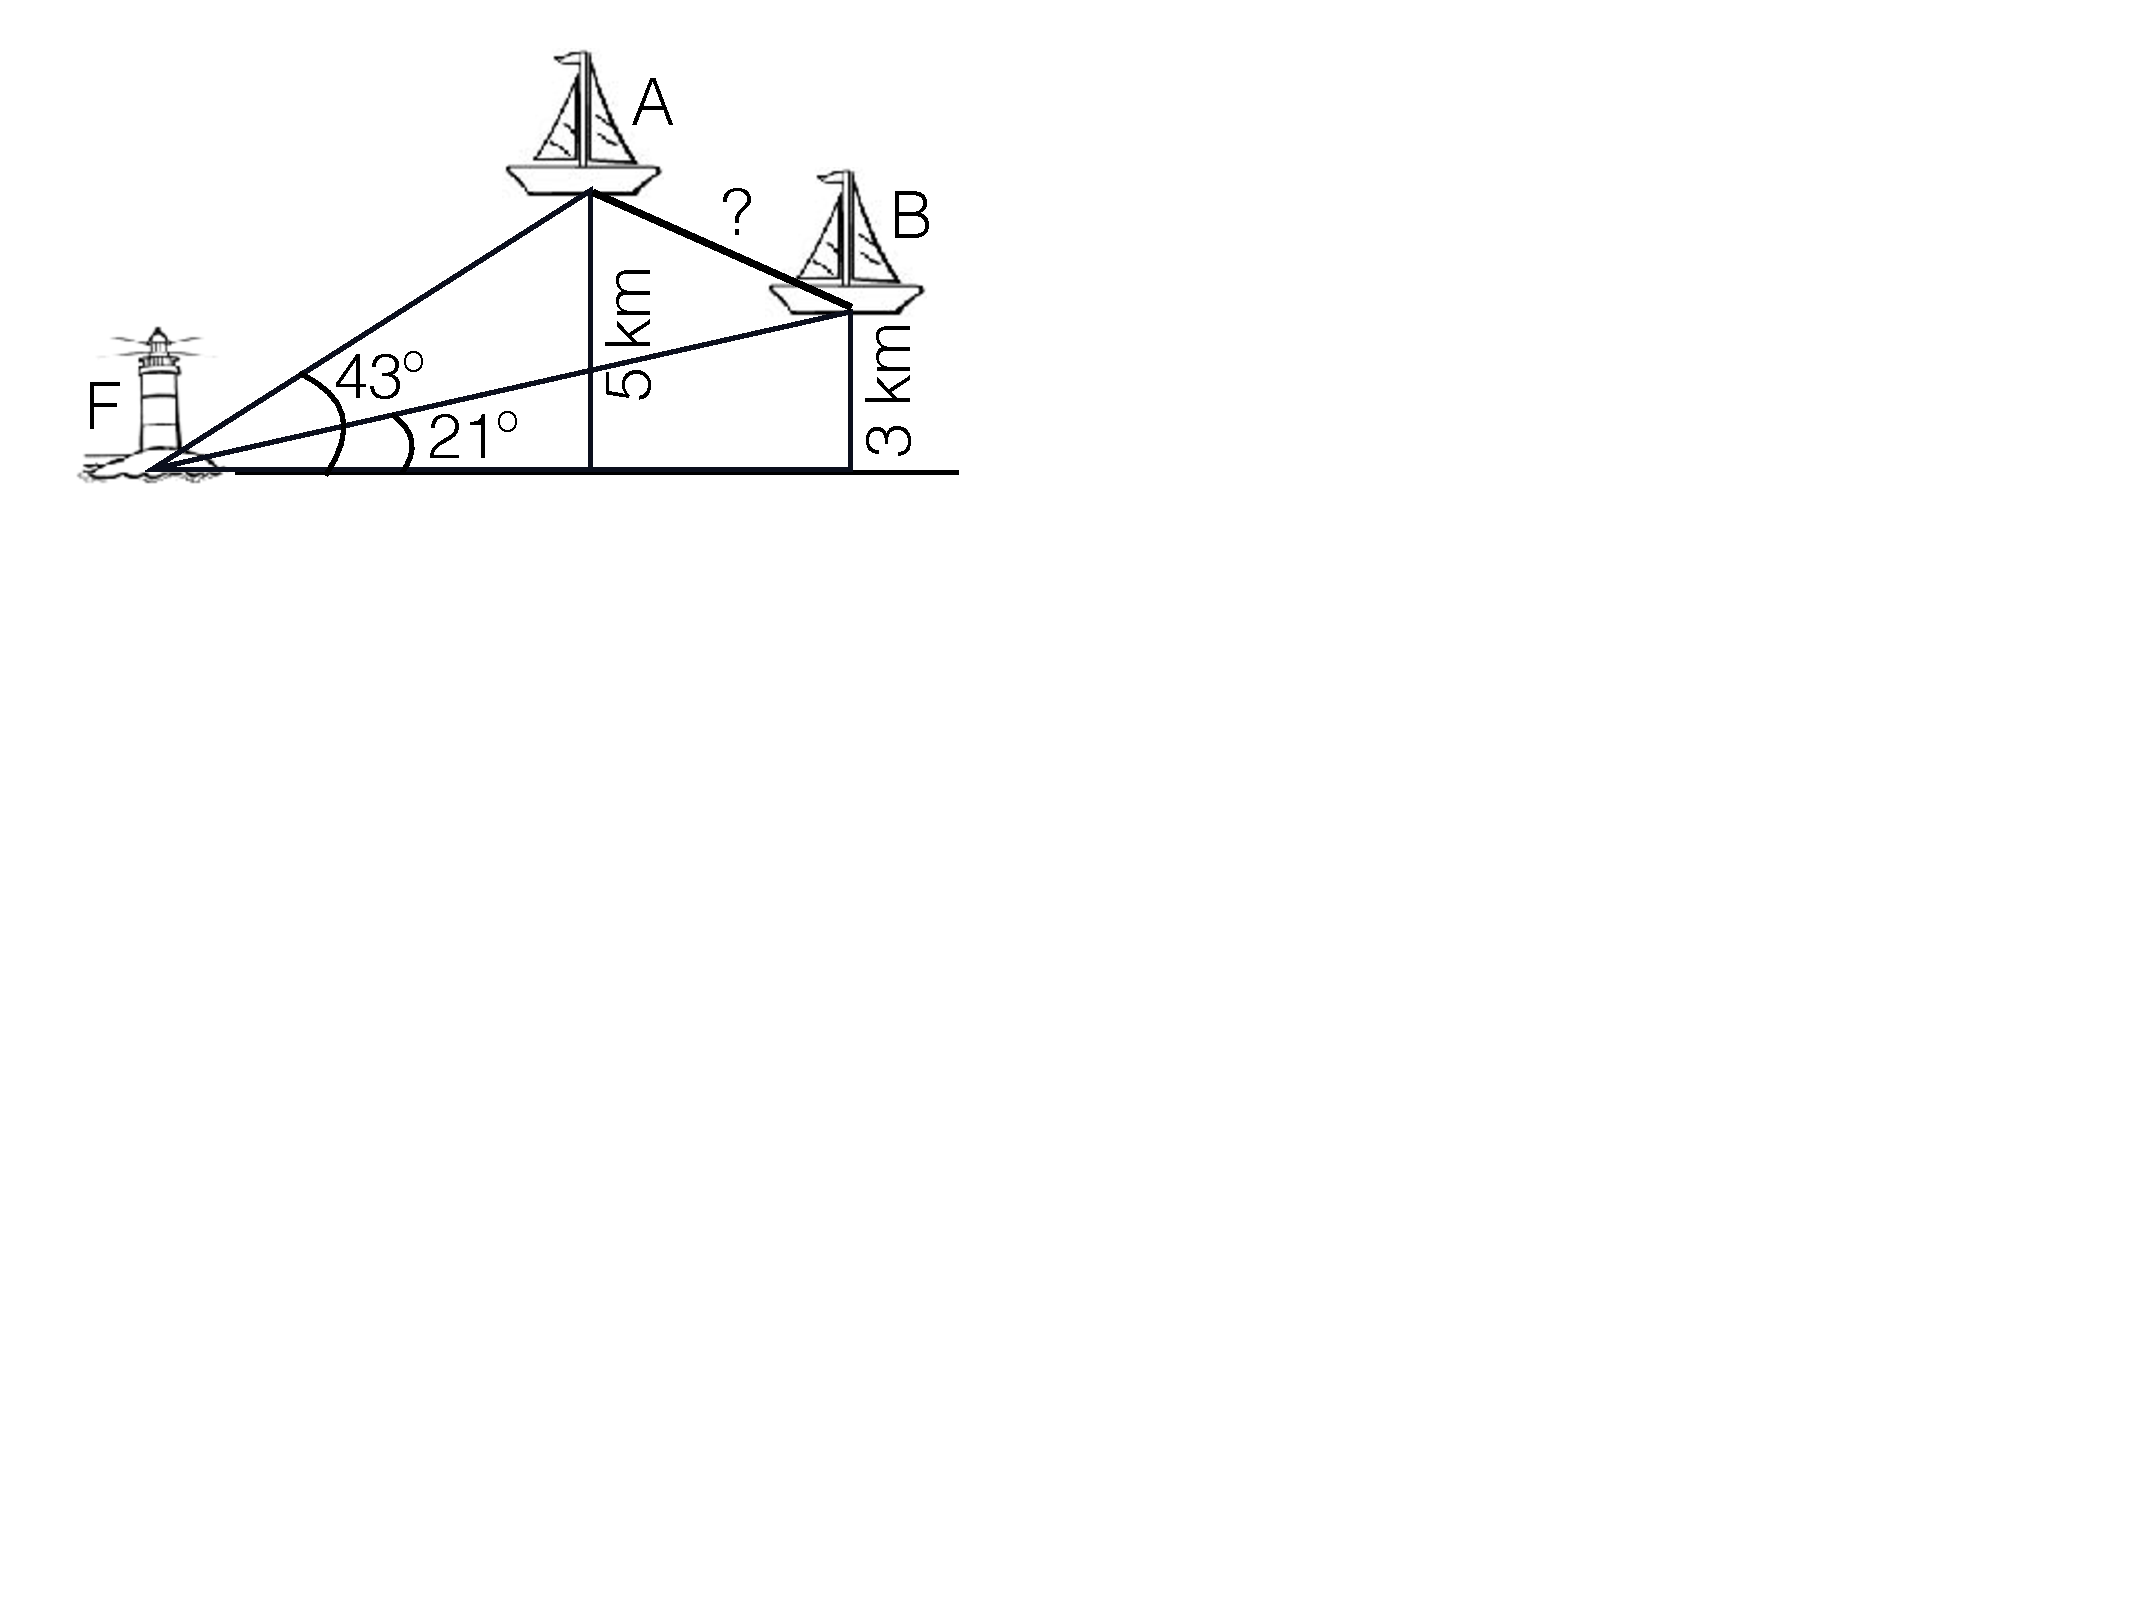
\includegraphics[width=5.1cm]{img-03/far}
	\end{center}
	
	\answers{Construïm el triangle rectangle de la figura. Té de catets $c=5-3=2$ i $b=\dfrac{3}{\tg 21} - \dfrac{5}{\tg 43}=2.453$. La distància és la hipotenusa del triangle $a=\sqrt{b^2+c^2}=3.165$ km 
		\par
			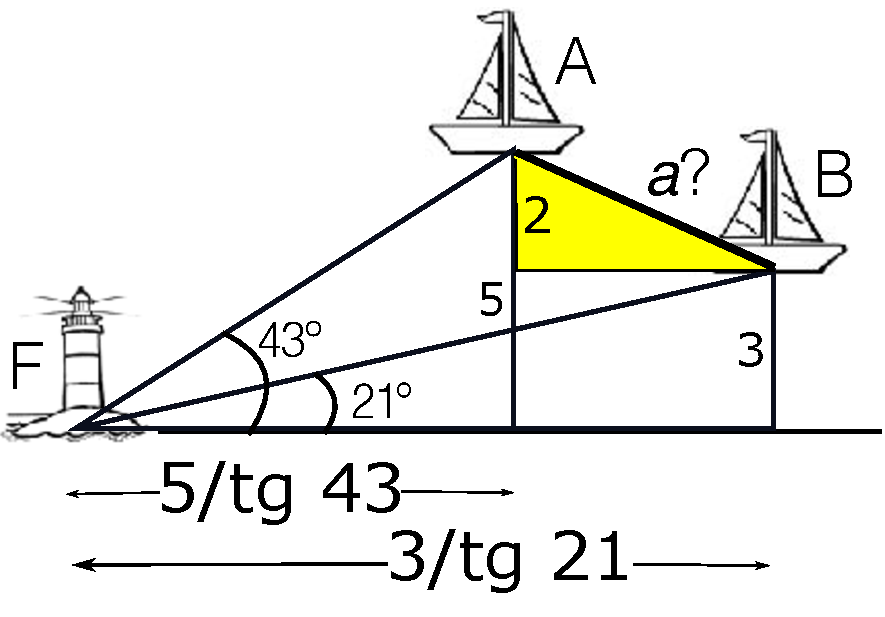
\includegraphics[width=0.4\textwidth]{img-sol/t3-37}
	}
	
	\exer
	Una finca té forma triangular. Dos dels seus costats mesuren 140 m i
	200 m respectivament, i l'angle comprès entre tots dos és de 35${}^\circ$.
	Calcula el perímetre i la superfície de la finca.
		\answers{Perímetre: 457.16 m. Àrea: 8030,1 m$^2$. 
		\par
		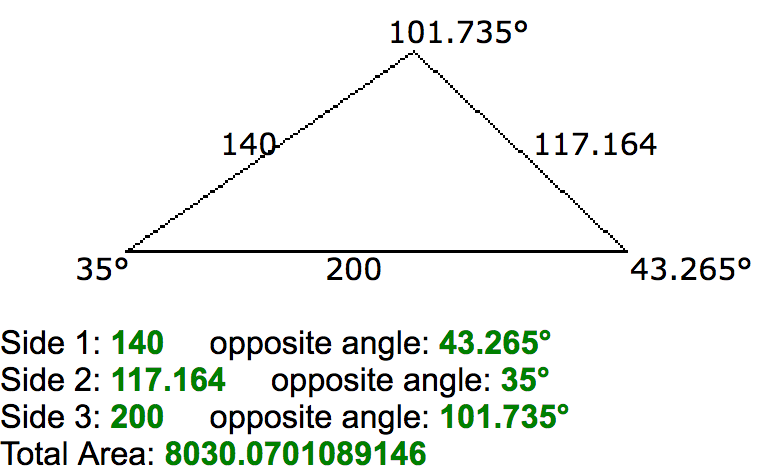
\includegraphics[width=0.42\textwidth]{img-sol/t3-38}
	}
	
	\exer
	Calcula l'altura de la torre: 
	\begin{center}
		\vspace{-1cm}
		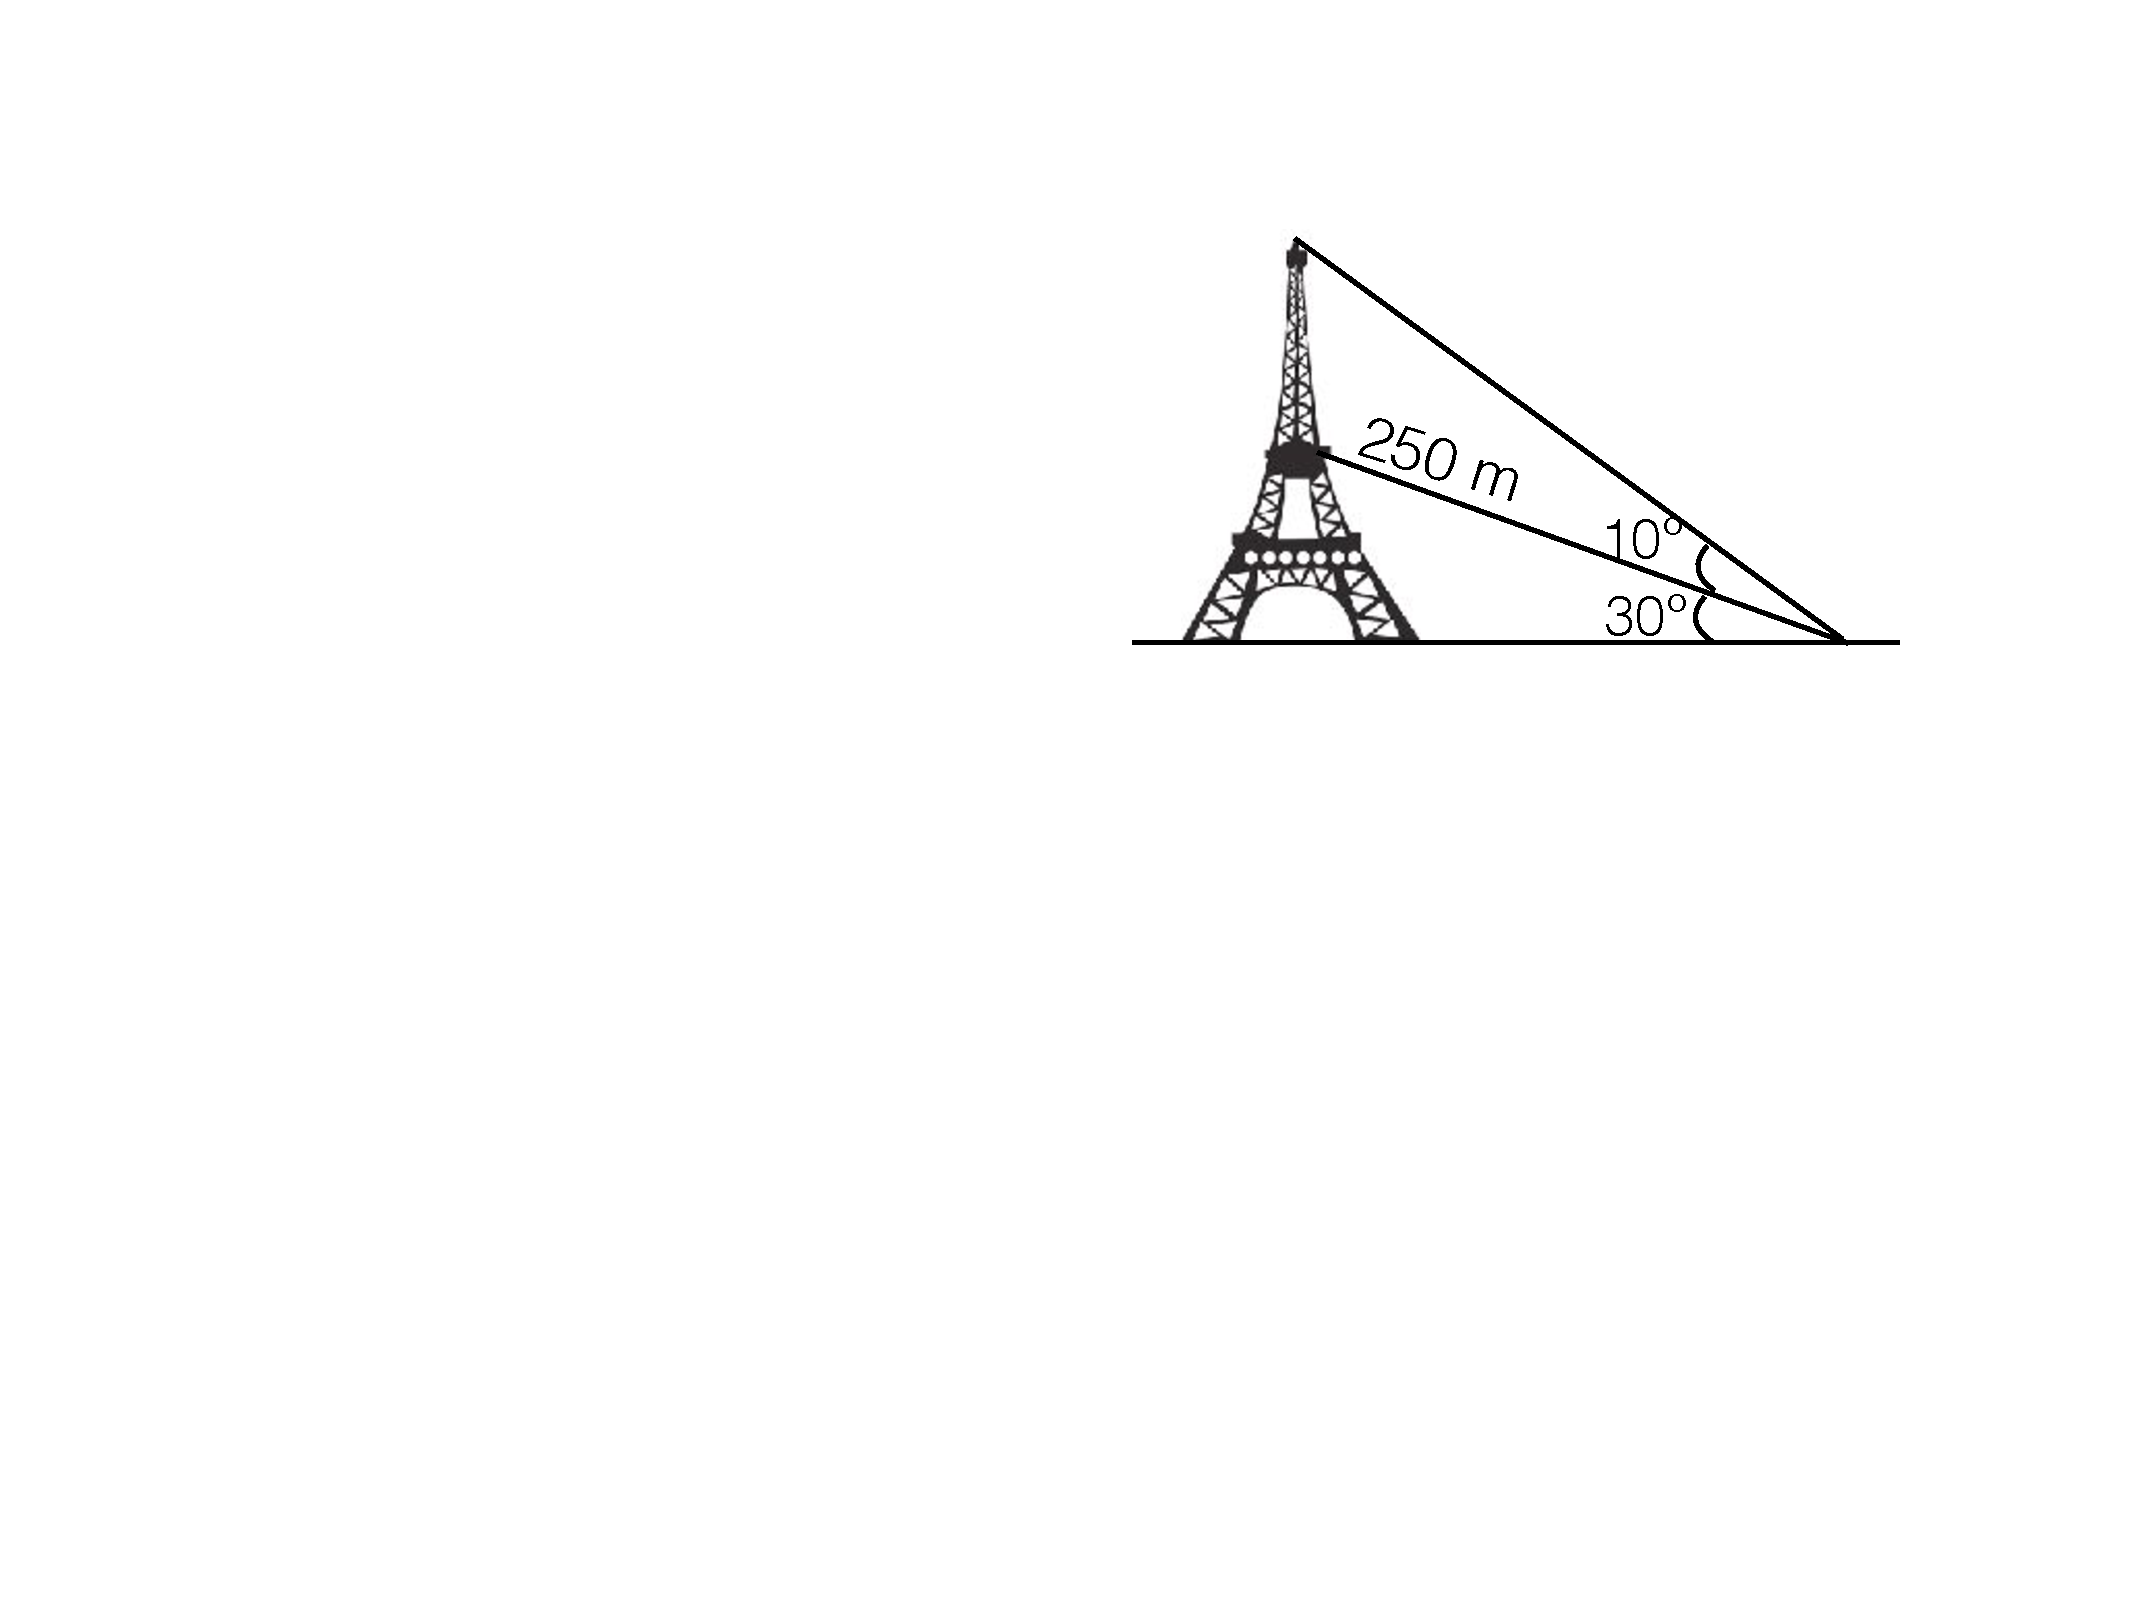
\includegraphics[width=5cm]{img-03/edifici}
	\end{center}

	\answers{Del triangle rectangle d'abaix trobam la base com $b=250\cos 30=216.51$ m. Del triangle rectangle complet $\tg 40 = \dfrac{H}{216.51}$, aïllam $H=181.67$ m.}
	
	\exer
	Dues persones \emph{A} \emph{i B} disten entre sí 200 m i veuen un
	globus que està situat entre ambdues. La primera persona ho veu amb un
	angle de 30${}^\circ$ i la segona amb un angle de 60${}^\circ$.
	
	\begin{tasks}
		\task
		A quina distància està \emph{B} del globus?
		\task
		A quina altura està el globus?
		\task
		Una persona que estigui situada dins del globus, amb quin angle veu
		a \emph{A} i \emph{B}?
	\end{tasks}
\answers[cols=3]{[100 m, 86.60 m, 90$^\circ$]}
	
	\exer
	\begin{minipage}[t]{0.55\textwidth}
		Calcula l'altura de la torre gran a partir del següent dibuix.
	\end{minipage}\hfill
	\begin{minipage}[t]{5.5cm}
		\vspace{-\baselineskip}
		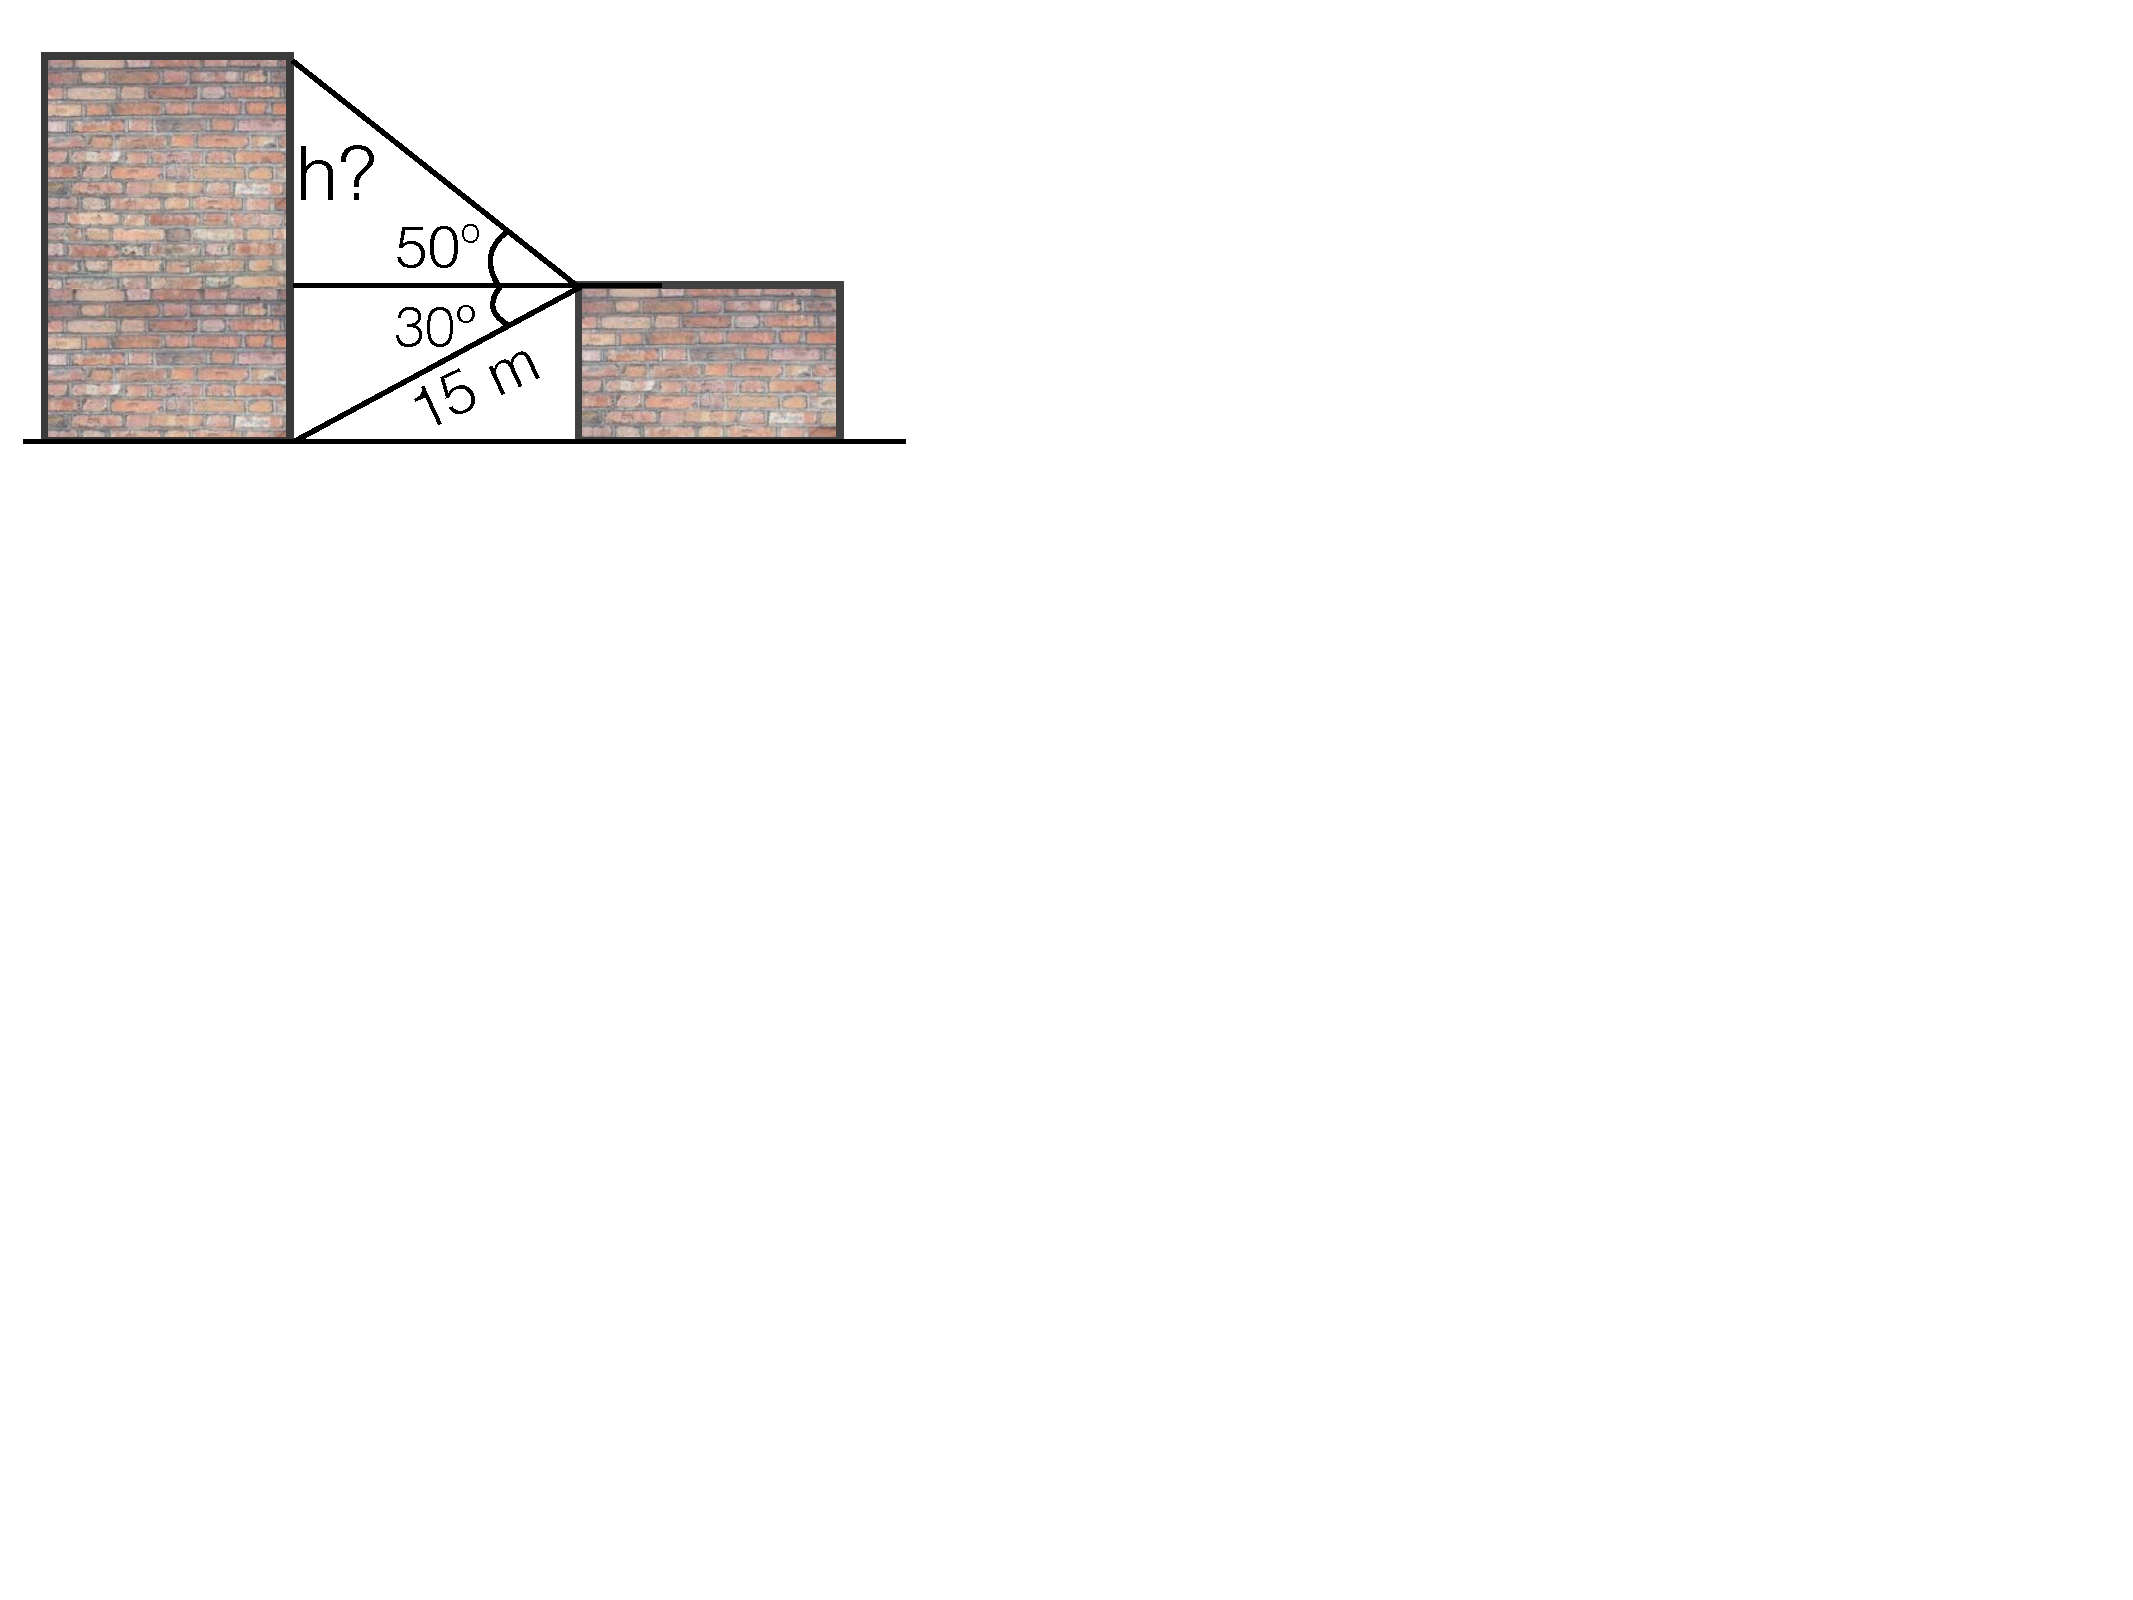
\includegraphics[width=5cm]{img-03/torre}
	\end{minipage}

	\answers{Primer trobam els angles que falten. Es un triangle d'angles 80, 60, 40. Aplicam el teorema del sinus: $\dfrac{h}{\sin 80}=\dfrac{15}{\sin 40}$. Aïllam $h =22.98$ m.}
	
	
	\exer
	Desitgem mesurar l'altura d'un edifici. Si ho observem des d'un punt
	\emph{A} ho veiem amb un angle de 50${}^\circ$. Ara bé, si ho contemplem des de
	20 m més lluny \emph{B}, l'angle és de 40${}^\circ$. Quina és l'altura de l'edifici? A
	quina distància està el punt \emph{B} d'aquest edifici?
	\answers{$d(B, E) = 67.59$; $h = 56,7135$ m}
	
	
	\exer
	Comencem en una ciutat \emph{A} i observem un cartell. La ciutat
	\emph{B} està a 50 Km i la ciutat \emph{C} a 40 Km. Mesurem l'angle
	que formen les dues carreteres i resulta ser de 60${}^\circ$. A quina distància
	està \emph{B} de C ? Des de la ciutat \emph{B}, amb quin angle es veuen
	les altres dues ciutats? {[}En altres paraules: si considerem el
	triangle \emph{ABC,} què val l'angle que correspon al vèrtex
	\emph{B}?{]}
	
	\answers{Des de $B$ les altres dues ciutats es veuen amb un angle de  49.11$^\circ$.
		\par
		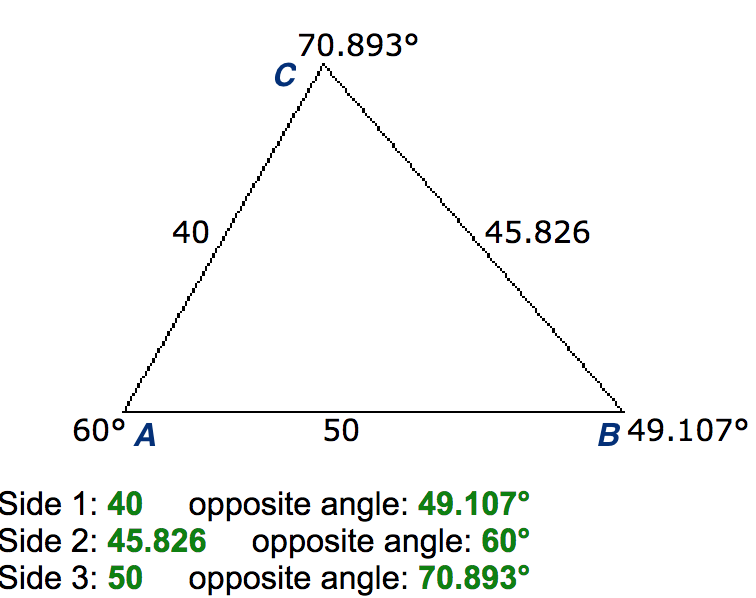
\includegraphics[width=0.43\textwidth]{img-sol/t3-43}}
	
	
	\exer[1] Per determinar l'amplada d'un riu ens fixam amb un 
	arbre que està situat en un punt C de la vorera. Arran de l'altra vorera
	hi ha dues cases A i B separades 30 m. Des de la casa A, l'arbre i la casa B
	formen un angle de 60${}^\circ$. Des de la casa B, l'angle que forma l'arbre i la casa A 
	és de 75${}^\circ$. Calcula l'amplada del riu. 
	\answers{$d=35,49$ m}
	
	\exer[-1]
	\begin{minipage}[t]{0.55\textwidth}
		\spicy  A i B són dues ciutats situades a l'altra banda d'un riu de pas 
		inaccessible. Aquestes ciutats, però, són visibles des d'altres punts accessibles
		C i D, separats per una distància de 73,2 km. Sabent els angles
		$\widehat{ACD}=80,2^\circ$, $\widehat{BCD}=43,5^\circ$, $\widehat{ADC}=23,23^\circ$, $\widehat{BDC}=32^\circ$, determina la distància entre les dues ciutats AB.
	\end{minipage}\hfill
	\begin{minipage}[t]{5.5cm}
		\vspace{-\baselineskip}
		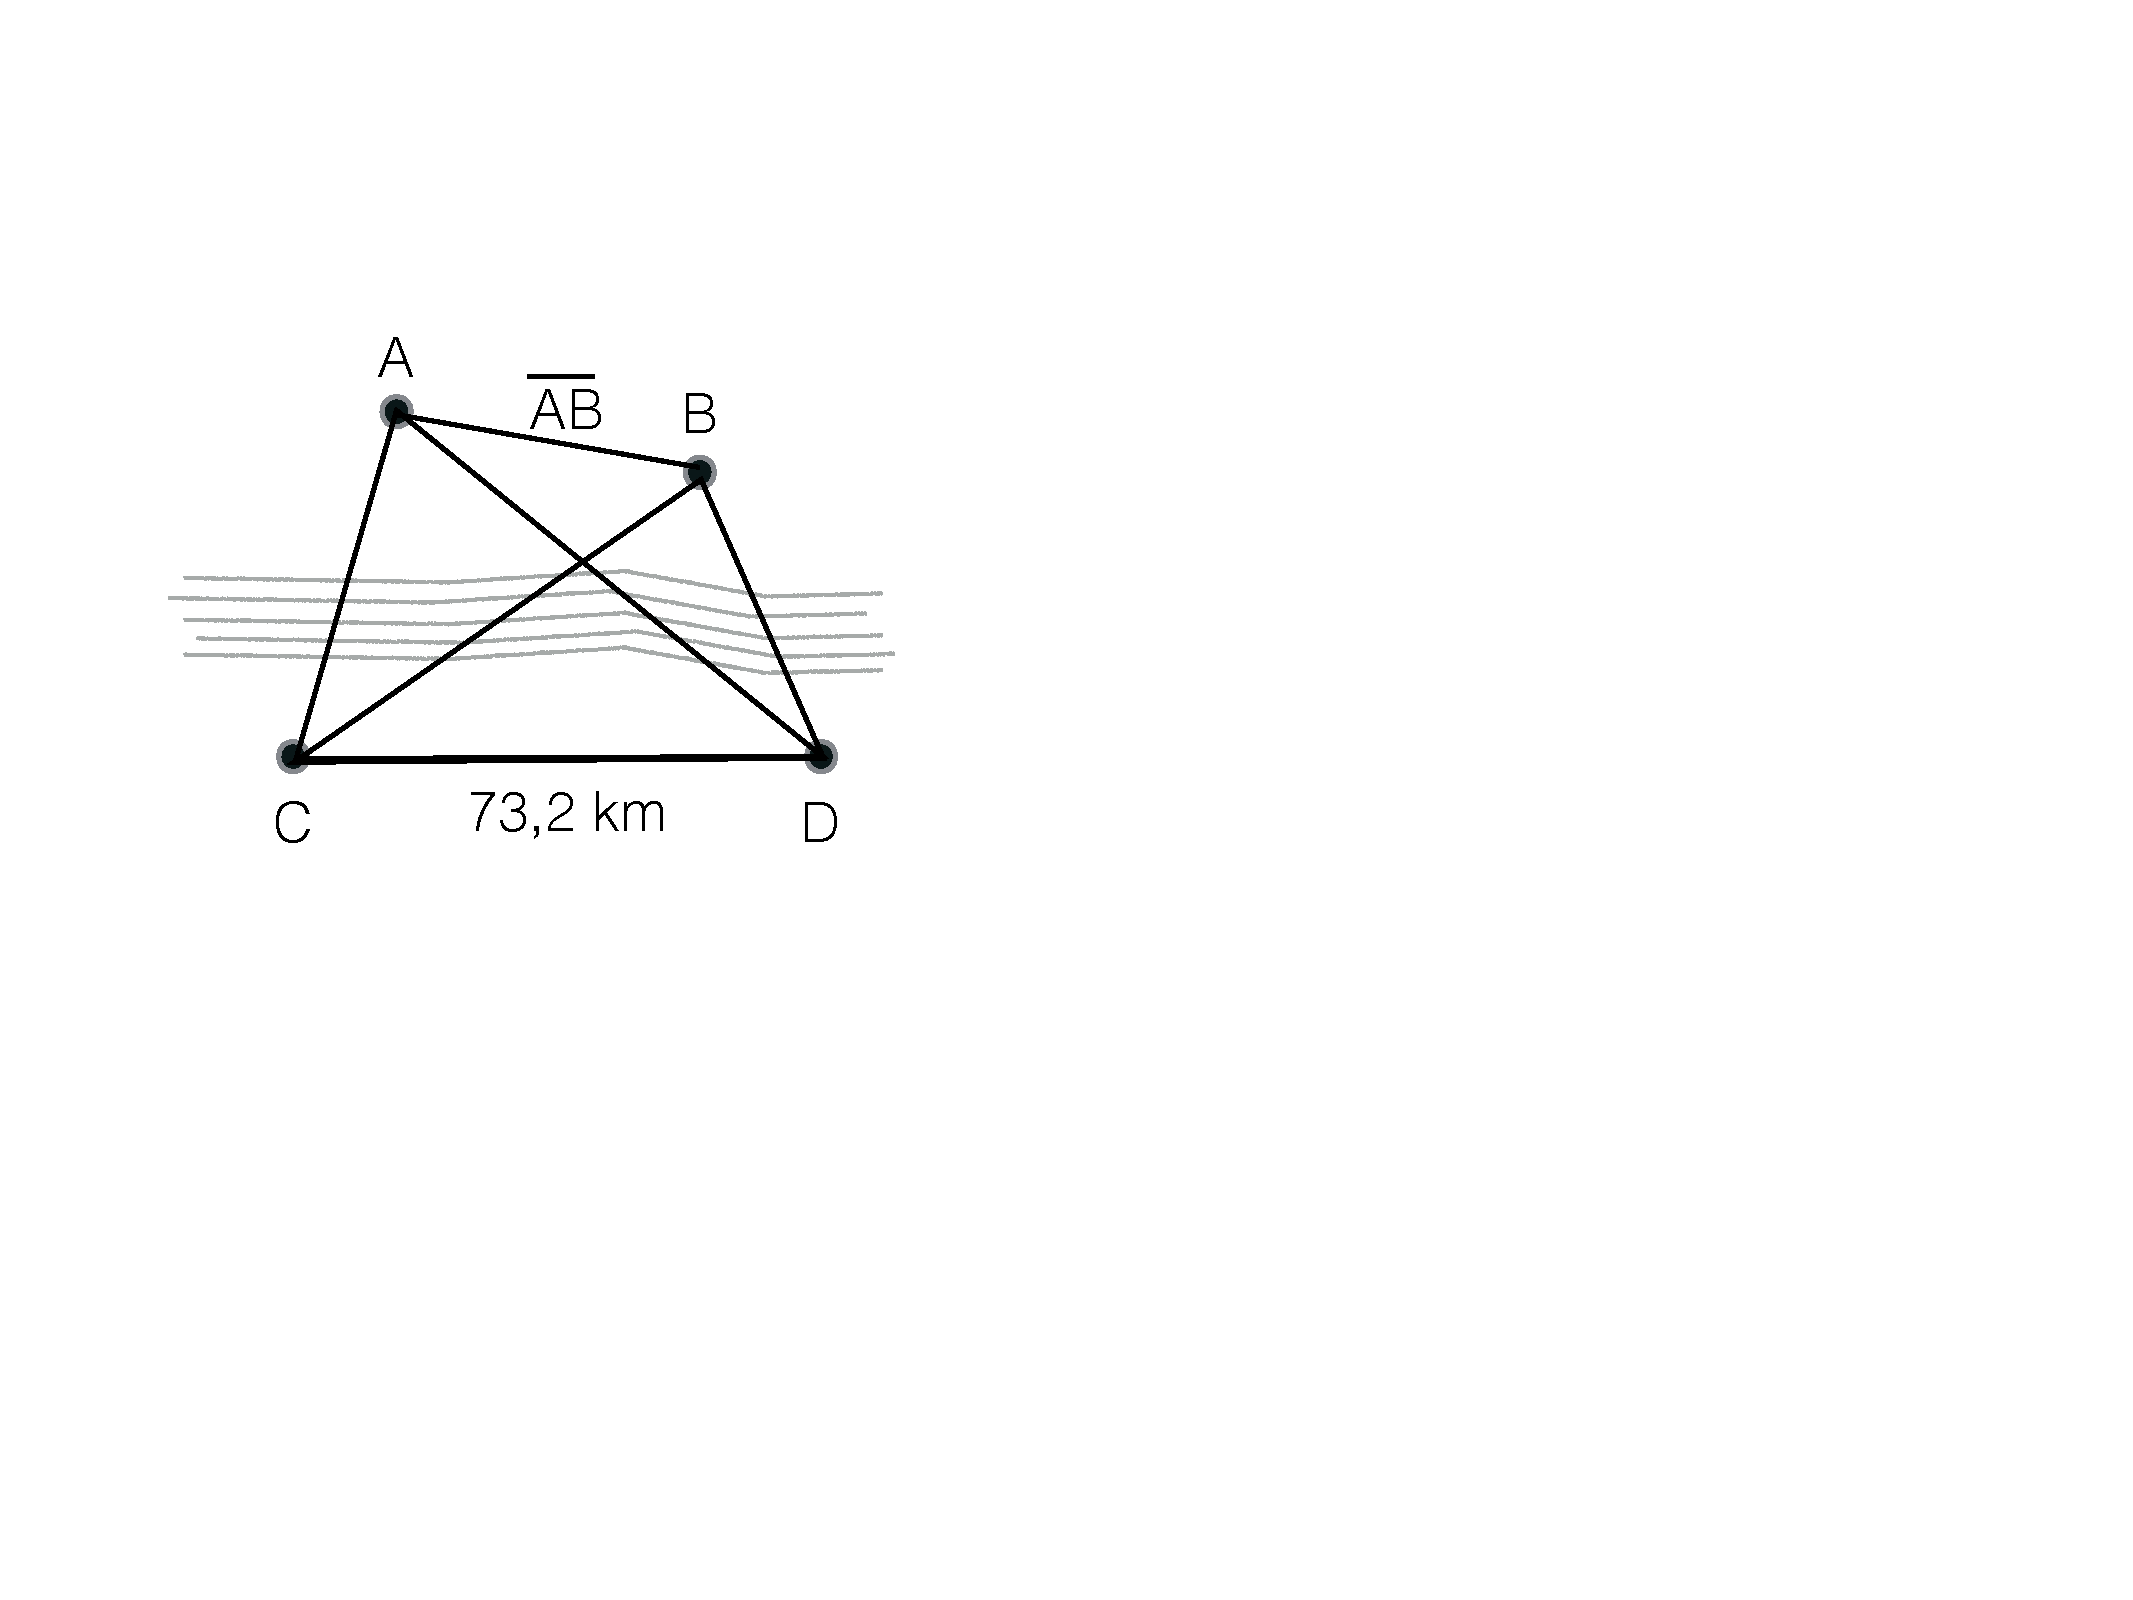
\includegraphics[width=5cm]{img-03/ciutats}
	\end{minipage}
	\answers{Del triangle $\widehat{CAD}$ troba $\overline{AD}=74.16$ km, del triangle $\widehat{CBD}$ troba $\overline{BD}=52.05$ km pel teorema del sinus i finalment del triangle $\widehat{ADB}$ troba  $\overline{AB}=24$ km pel teorema del cosinus.}
	
	\exer[1]
	\begin{minipage}[t]{0.55\textwidth}
		\spicy Dos muntanyistes que han pujat en caps de setmana successius a dos cims veïns volen saber quina és la
		distància entre aquests dos cims. Per això, han mesurat des del peu del cim A els angles d'elevació dels cims A i B que són 65${}^\circ$ i 30${}^\circ$, respectivament. 
	\end{minipage}\hfill
	\begin{minipage}[t]{5.5cm}
		\vspace{-\baselineskip}
		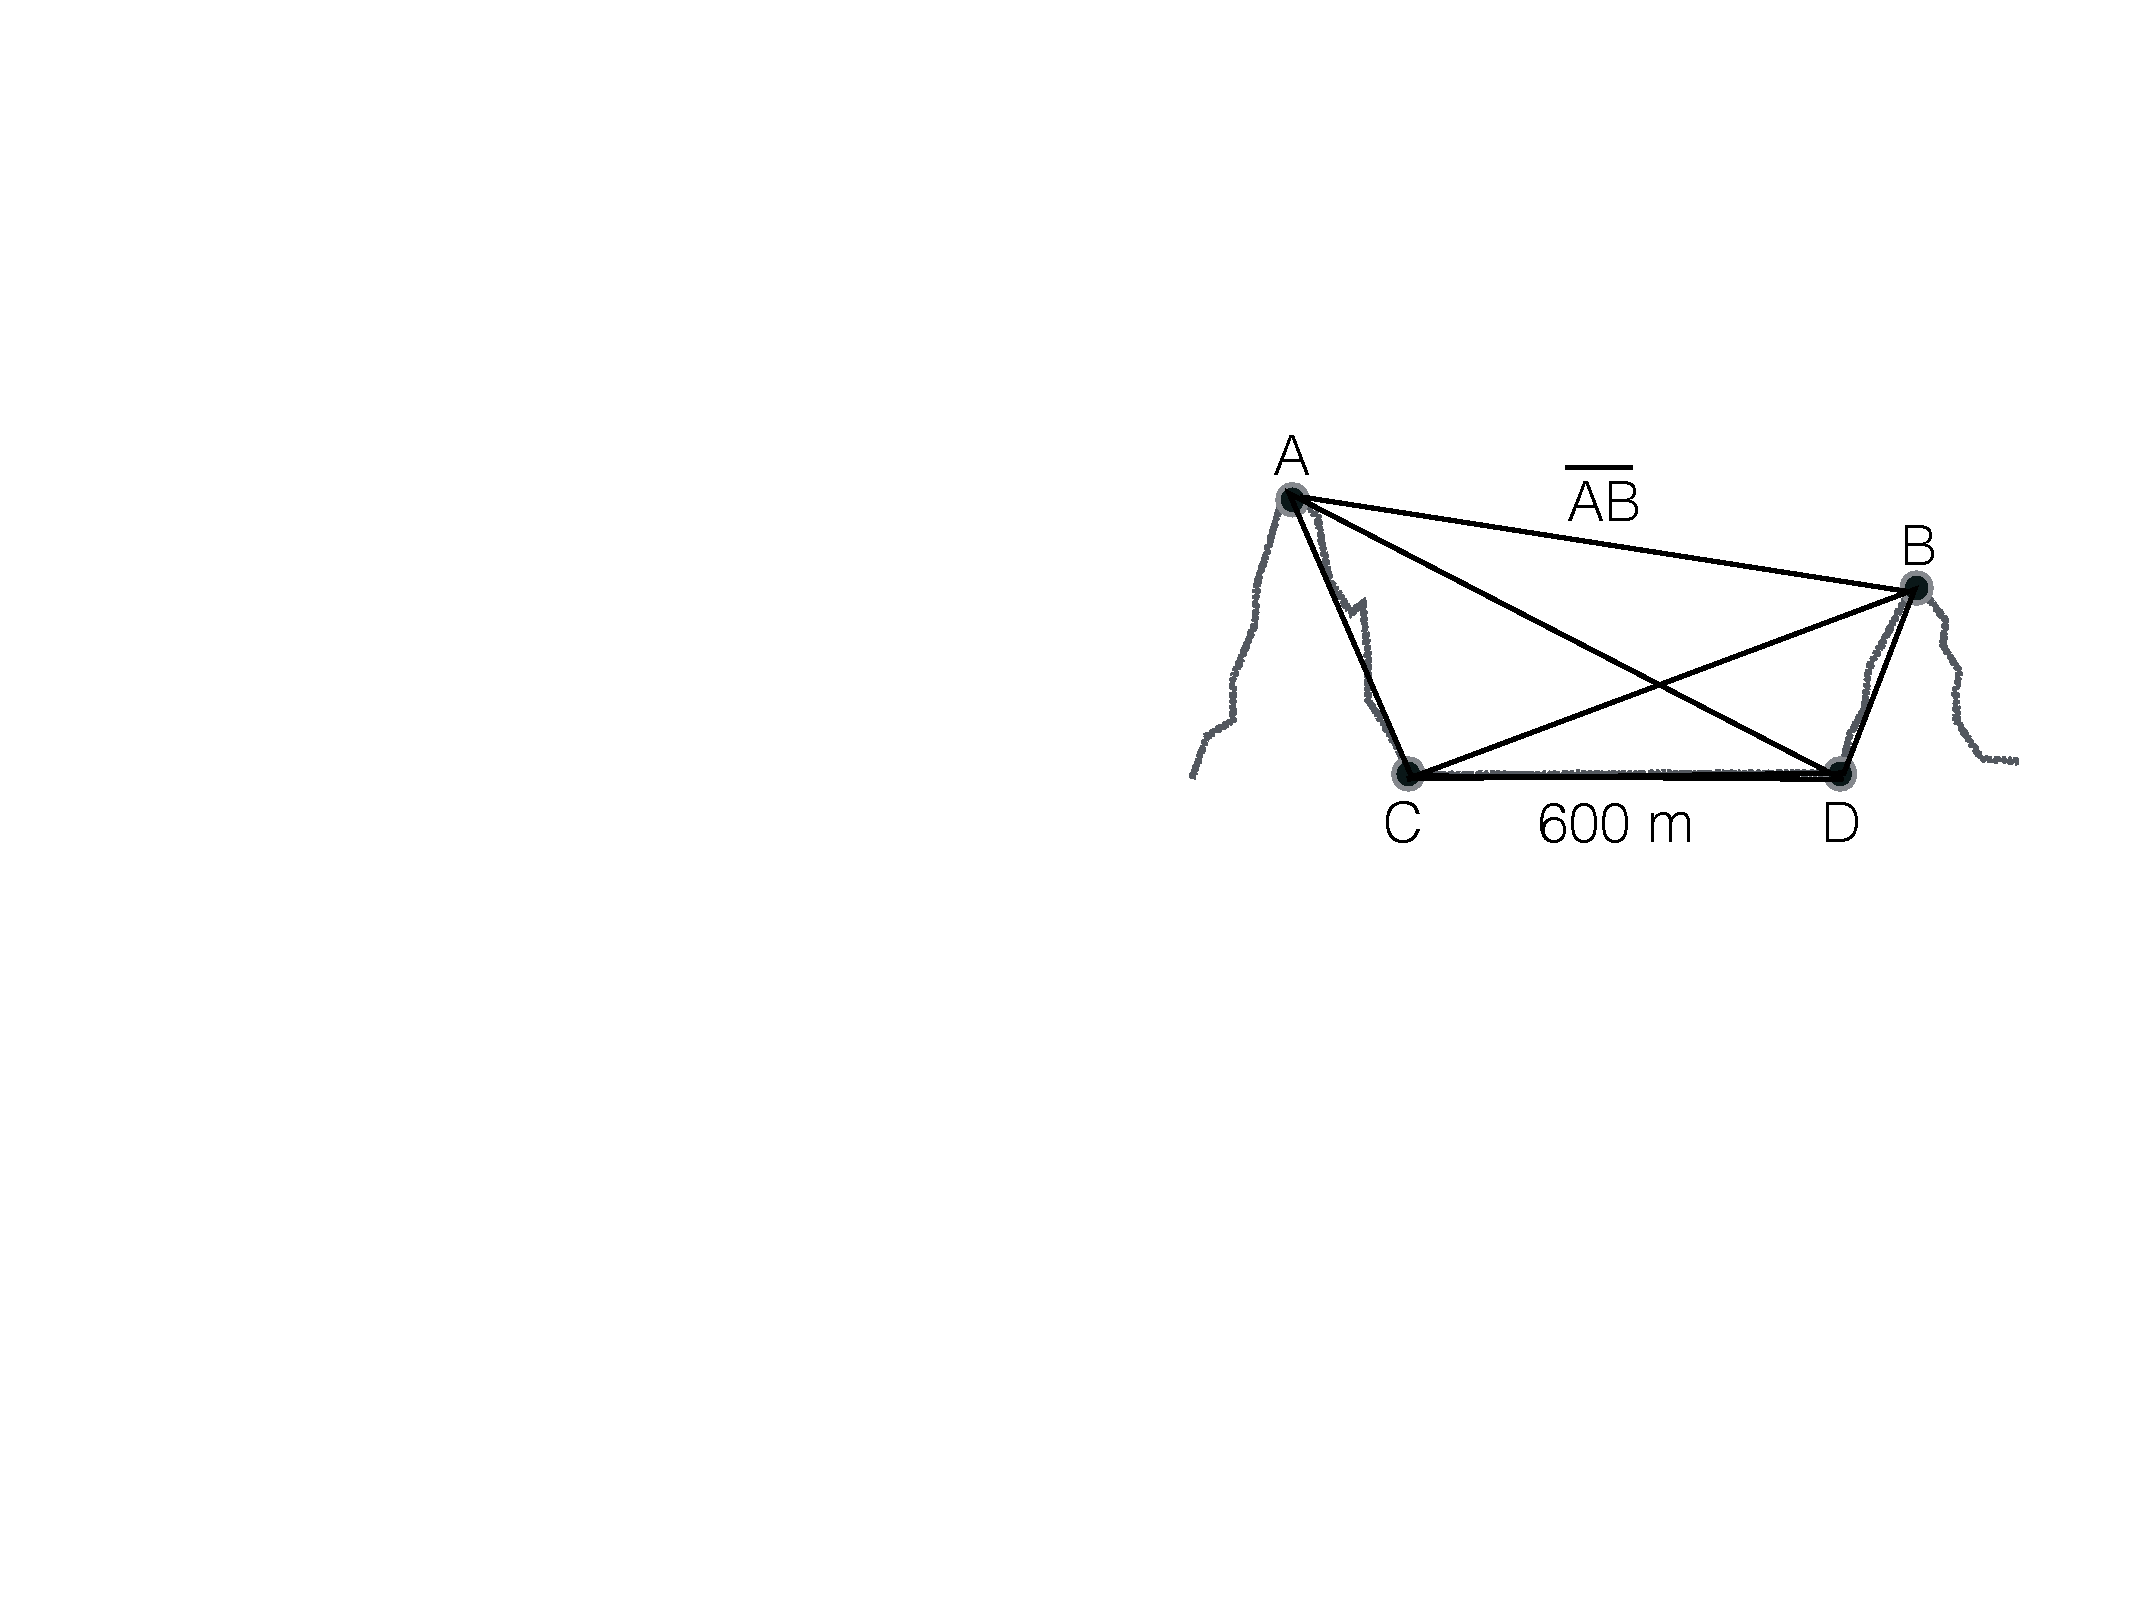
\includegraphics[width=5.3cm]{img-03/muntanyes}
	\end{minipage}
	
	Després han caminat fins el peu del cim B i han mesurat els angles d'elevació dels cims A i B de 40${}^\circ$ i 47${}^\circ$, respectivament. La distància entre els dos peus dels cims és de 600 m. Què val la distància entre els dos cims?
	\answers{cim A=827 m, cim B=751 m, distància entre cims AB=1687.2 m}

	\exer
	En un viatge d'alumnes de 4t d'ESO a Londres, alguns dels viatgers
	van fer pràctiques de trigonometria. En conèixer que
	l'Abadia de Westminster té una altura de 30 metres, van decidir
	aprofitar els seus coneixements per calcular l'altura de la famosa
	torre Big Ben. Des d'un punt situat entre els dos edificis
	s'observa el punt més alt de l'Abadia amb angle de 60$^\circ$, i el Big Ben
	amb un angle de 45$^\circ$. Si la distància entre les bases de les torres
	dels dos edificis és de 50 metres, quin va ser el resultat dels seus
	càlculs?, a quina distància es trobava de cada edifici?
	
	\answers{Es trobava a 17.32 m de l'Abadia de Westminster i a 32.68 m del Big Ben. L'altura del Big Ben és 32.68 m ja que es veu amb un angle de 45$^\circ$.
	\par 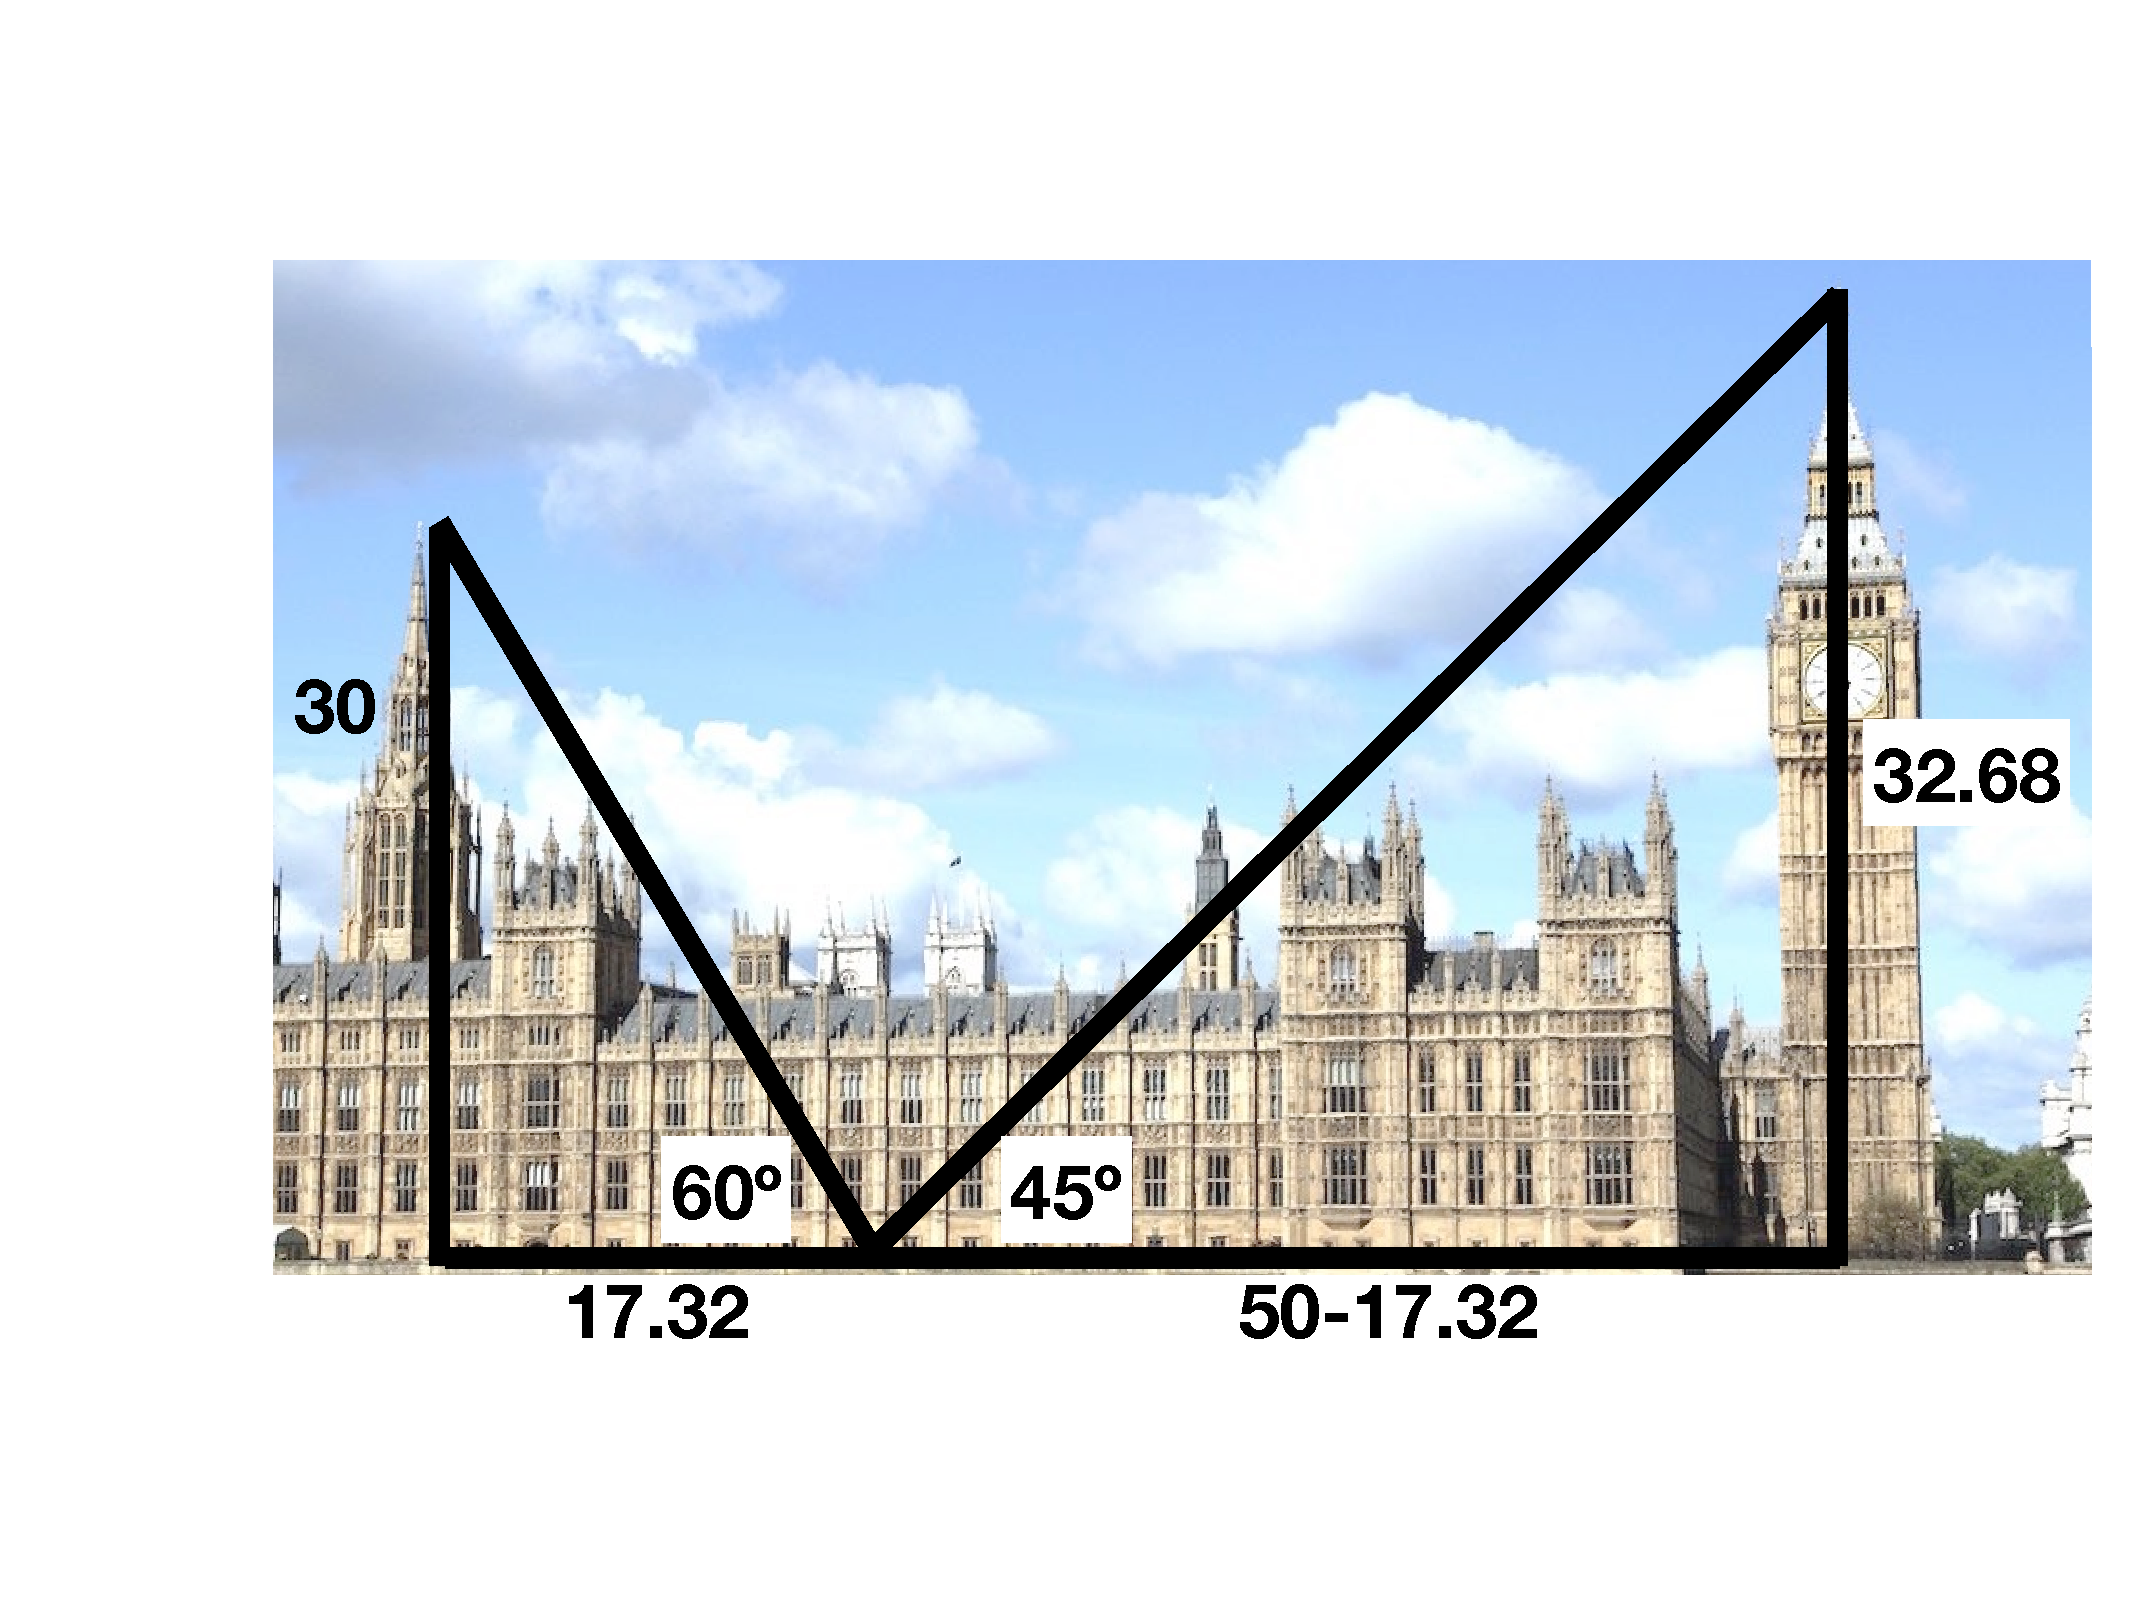
\includegraphics[width=0.4\textwidth]{img-sol/t3-47}}
\end{mylist}

\section{Identitats trigonomètriques}

\begin{theorybox}{Trobareu un resum de les identitats trigonomètriques a la pàgina \pageref{sec:formularitrig}.}
	\vspace{0.4cm}
	
	\begin{minipage}{0.25\textwidth}	
		\centering
		\videonw{145}{Identitats  1: Suma d'angles}
		
	\end{minipage}
	\begin{minipage}{0.25\textwidth}
		\centering
		\videonw{146}{Identitats  2: Diferència d'angles}
		
	\end{minipage}
	\begin{minipage}{0.25\textwidth}
		\centering
		\videonw{148}{Identitats  3: Angle doble}
		
	\end{minipage}
	\begin{minipage}{0.25\textwidth}
		\centering
		\videonw{147}{Identitats  4: Relació de l'angle meitat}
		
	\end{minipage}
	
	\vspace{0.5cm}
\end{theorybox}

\begin{mylist}
	\exer
	Calcula a partir de les raons trigonomètriques de
	30${}^\circ$, 45${}^\circ$, 60${}^\circ$ i
	90${}^\circ$, les raons trigonomètriques de
	75${}^\circ$, 120${}^\circ$, 150${}^\circ$, 
	105${}^\circ$ i 135${}^\circ$
	
	\begin{example}[*]
		Per exemple, si utilitzam la relació de la suma d'angles i expressam $75^\circ =45^\circ + 30^\circ$
		
		$\sin(75^\circ)=\sin(45^\circ + 30^\circ)=\sin(45^\circ)\cdot \cos(30^\circ) + \cos(45^\circ)\cdot \sin(30^\circ)=\frac{\sqrt{2}}{2}\frac{\sqrt{3}}{2}+\frac{\sqrt{2}}{2}\frac{\sqrt{1}}{2}=\frac{\sqrt{6}+\sqrt{2}}{4}$
	\end{example}
	
	\begin{example}[*]	
		De forma similar, podem obtenir el cosinus
		
		$\cos(75^\circ)=\cos(45^\circ + 30^\circ)=\cos(45^\circ)\cdot \cos(30^\circ) - \sin(45^\circ)\cdot \sin(30^\circ)=\frac{\sqrt{2}}{2}\frac{\sqrt{3}}{2}-\frac{\sqrt{2}}{2}\frac{\sqrt{1}}{2}=\frac{\sqrt{6}-\sqrt{2}}{4}$
		
		i finalment, la tangent
		
		$\tg(75^\circ)=\tg(45^\circ + 30^\circ)=\dfrac{\tg 45^\circ + \tg 30^\circ}{1-\tg 45^\circ \cdot \tg 30^\circ}=\dfrac{1 + \frac{\sqrt{3}}{3}}{1-1 \cdot \frac{\sqrt{3}}{3}}=2+\sqrt{3}$
	\end{example}
	
	\exer
	Calcula a partir de les raons trigonomètriques de
	30${}^\circ$, 45${}^\circ$, 60${}^\circ$ i
	90${}^\circ$, les raons trigonomètriques de
	15${}^\circ$
	
	\answers{15=45-30; $\sin 15=\sin 45\cos 30 - \cos 45 \sin 30= \dfrac{\sqrt{6}-\sqrt{2}}{4}$ \par $\cos 15=\cos 45\cos 30 + \sin 43 \sin 30= \dfrac{\sqrt{6}+\sqrt{2}}{4}$ \par $\tg 15=2-\sqrt{3}$ }
	
	\exer
	Comprova que les raons trigonomètriques de 30${}^\circ$ es
	poden obtenir a partir de les raons trigonomètriques de 90${}^\circ$, 
	i de 60${}^\circ$.
	
	\answers{30=90-60; $\sin 30=\sin 90\cos 60 - \cos 90 \sin 60= \cos 60 = \dfrac{1}{2}$ \par $\cos 30=\cos 90\cos 60 + \sin 90 \sin 60= \sin 60 =\dfrac{\sqrt{3}}{2}$ \par $\tg 60=\sqrt{3}$ }
	
	
	\exer
	Demostra les fórmules d'angles complementaris ($90-\alpha$) emprant les fórmules de la
	diferència: $\sin(90-\alpha)=\cos\alpha$, $\cos(90-\alpha)=\sin\alpha$ i $\tg(90-\alpha)=1/\tg\alpha$.
	
	\answers{$\sin(90-\alpha)=\sin 90 \cos \alpha - \cos 90 \sin \alpha = \cos \alpha$,\par $\cos(90-\alpha)=\cos 90 \cos \alpha + \sin 90 \sin \alpha=\sin\alpha$ i $\tg(90-\alpha)= 1/\tg\alpha$}
	
	\exer
	Calcula les raons trigonomètriques de
	22'5${}^\circ$ i 11'25${}^\circ$ a partir de les
	raons trigonomètriques de 45${}^\circ$.
		
	\answers{$22.5 = 45/2$, $\sin 22.5= \dfrac{\sqrt{2-\sqrt{2}}}{2}$, $\cos 22.5= \dfrac{\sqrt{2+\sqrt{2}}}{2}$, $\tg 22.5= \sqrt{3-2\sqrt{2}}$\par
		$11.25 = 22.5/2$, $\sin 11.25= \frac{\sqrt{2-\sqrt{2+\sqrt{2}}}}{2}$, $\cos 11.25= \frac{\sqrt{2+\sqrt{2+\sqrt{2}}}}{2}$, $\tg 11.25= -1-\sqrt{2}+\sqrt{2(2+\sqrt{2})}$
	}
	
	
	
	\exer
	Comprova que les raons trigonomètriques de 45${}^\circ$ es
	poden obtenir a partir de les raons trigonomètriques de 90${}^\circ$.
	\answers{$45 = 90/2$, $\sin 45= \sqrt{\frac{1-\cos 90}{2}}=\frac{\sqrt{2}}{2}$, $\cos 45= \sqrt{\frac{1+\cos 90}{2}}=\dfrac{\sqrt{2}}{2}$,\par $\tg 45= \sqrt{\dfrac{1-\cos 90}{1+\cos 90}}=1$}
	
	
	\exer[-1] Demostra $\sin^2 \alf \cdot \cos \alf + \cos^3 \alf= \cos \alf$. 
	\answers{Treu factor comú $\cos \alpha$ i utilitza la relació fonamental.}
	
	\end{mylist}
	
	\begin{example}
		Per fer una demostració d'una identitat cal partir del terme de l'esquerre i, aplicant altres relacions que sabem que són certes, arribar al terme de la dreta que volem demostrar. 
		
		Així doncs, en aquest exemple partirem de $\sin^2 \alf \cdot \cos \alf + \cos^3 \alf$ i treurem factor comú $\cos \alf$, obtenint
		
		$\sin^2 \alf \cdot \cos \alf + \cos^3 \alf = \cos\alf \cdot (\sin^2 \alf + \cos^2 \alf)$ ara utilitzam la relació fonamental que diu que $\sin^2 \alf + \cos^2 \alf=1$, aleshores trobam $\sin^2 \alf \cdot \cos \alf + \cos^3 \alf = \cos\alf$ que era el resultat que voliem demostrar (\textbf{c.v.d.}).
		
	\end{example}
	
	
	\begin{mylist}
		
	\exer[-1] Demostra $(\sin \alf + \cos \alf)^2 = 1 + \sin 2\alf$. 
	\answers{Desenvolupa el quadrat amb la identitat notable $(a+b)^2 = a^2 + b^2 + 2ab$. Empra la relació fonamental i la fórmula de $\sin 2\alf$.}
	
	\exer[-1] Demostra $2\sin x + \cos(-x)-\sin(-x)-\cos x = 3 \sin x$. 
	\answers{Utilitza les relacions de l'angle oposat $\cos(-x)=\cos x$, $\sin(-x)=-\sin x$, $\tg(-x)=-\tg x$.}
	
	\exer[-1] Demostra $\tg \alf + \cotg \alf = \sec \alf \cdot \cosec \alf$. 
	\answers{Expressa $\tg \alf$ i $\cotg \alf$ com a quocients de sinus i cosinus. Després realitza la suma de fraccions amb el
	mínim comú múltiple. Finalment utilitza la relació fonamental.}
	
	\exer[-1] Demostra $\sin 3\alf = \sin\alf \cdot \left( 3\cos^2 \alf - \sin^2 \alf \right)$. 
	\answers{Escriu $\sin(3\alf) = \sin(\alf+2\alf)$. Aplica la fórmula de la suma d'angles i tot seguit les
	fórmules de l'angle doble. Finalment opera, simplifica i treu factor comú $\sin \alf$.}
	
	\exer[-1] Demostra $\cos 4\alf = \cos^4\alf+\sin^4\alf-6\sin^2 \alf \cos^2 \alf$. 
	\answers{Escriu $\cos(4\alf) = \cos(2\alf+2\alf)$. Aplica la fórmula de la suma d'angles i tot seguit les
	fórmules de l'angle doble. Finalment opera i simplifica.}
	
	
	\exer Simplifica les següents expressions:
	\begin{tasks}(2)
		\task $(\sin x + \cos x)^2 + (\sin x - \cos x)^2$
		\task $\dfrac{\sin(2 a)\cdot \cos a}{\sin a \cdot (1+\cos(2 a))}$
		\task $\dfrac{\sin^3 x+\sin x \cdot \cos^2 x}{\sin x}$
		\task $\dfrac{\sin(x-y)-\sin(x+y)}{\cos(x+y)-\cos(x-y)}$
	\end{tasks}
\answers{[2, 1, 1, $\cotg x$]}
	
	
%	\exer
%	Comprova si són certes o falses les següents igualtats: 
%	\begin{tasks}(2)
%		\task $\dfrac{1+\tg^{2} x}{1+\cotg^{2} x} =\tg^{2} x$
%		\task $\dfrac{\sin\left(2x\right)}{1+\cos \left(2x\right)} =\tg x$
%	\end{tasks}


	\exer
	Demostra que són certes les següents igualtats: 
	\begin{tasks}(2)
		\task $\dfrac{2\sin x}{\tg 2x} =\cos x-\dfrac{\sin^{2} x}{\cos x} $
		\task $\dfrac{1-\sin^{4} x}{\cos ^{2} x} =2-\cos ^{2} x$
	\end{tasks}
	\exer
	Comprova que són certes les següents igualtats: 
	\begin{tasks}(2)
		\task $\dfrac{1+\tg^{2} \alpha }{1+\cotg^{2} \alpha } =\tg^{2} \alpha $
		\task $\dfrac{\cos ^{2} \alpha }{1+\sin\alpha } =1-\sin\alpha $
	\end{tasks}
	
	\exer
	Utilitza les transformacions de sumes en productes per posar en funció
	del sinus i cosinus de l'angle $a$:
	
	\begin{tasks}(2)
		\task $\sin(45+a) + \sin(45 -a)$
		\task $\cos(120+a) + \cos(60 + a)$
	%	\task $\cos(270- a ) - \cos(90 - a)$
	\end{tasks}

\answers{[$\sqrt{2}\sin a$, $-\sqrt{3}\sin a$]}
	
	
	\exer
	Demostra les següents identitats:
	\begin{tasks}(2)
		\task $\tg x \cdot \cos x = \sin x$
		\task $1+\tg^2 x = \sec^2 x$
		\task $1+\cos 2x = \dfrac{2}{1+\tg^2 x}$
		\task $\dfrac{\cos x + \sin x}{\cos x - \sin x}\cdot \cos 2x = 1 + \sin 2x$
	\end{tasks}
	
\end{mylist}



\section{Equacions i sistemes trigonomètrics}

 \begin{warningbox}
	\begin{multicols}{2}
		
		\heading{Identitat}:  $\mathbf{(x+1)^2=x^2+2x+1}$
		
		{\footnotesize És certa sempre, per qualsevol $x$}
		
		\columnbreak
		
		\heading{Equació}: $\mathbf{x^2 -x =2}$
		
		{\footnotesize Volem trobar els valors de $x$ pels quals es compleix $=$}
	\end{multicols}
\end{warningbox}

\begin{theorybox}
	\begin{minipage}{0.33\textwidth}
		\centering
		\videonw{138}{Equacions trigonomètriques nivell 1}
	\end{minipage}
	\begin{minipage}{0.33\textwidth}
		\centering
		\videonw{139}{Equacions trigonomètriques nivell 2}
	\end{minipage}
	\begin{minipage}{0.33\textwidth}
		\centering
		\videonw{140}{Equacions trigonomètriques nivell 3}
	\end{minipage}
\end{theorybox}

\begin{mylist}
	\exer
	Resol les següents equacions trigonomètriques
	\begin{tasks}(3)
		\task $\cos x = -\frac{1}{2}$
		\task $\tg x = \sqrt{3}$
		\task $\sin x = -\frac{\sqrt{2}}{2}$
%%
		\task $\tg x = -1$
		\task $\cosec x = 4$
		\task $\cos x = \frac{1}{3}$
%%
		\task $\sin x = \cos x$
		\task $\tg^2 x = \frac{1}{3}$
		\task $\cos^2 x = \frac{1}{2}$
	\end{tasks}
\answers[cols=1]{[$x=120+n\cdot 360$ i $x=240+n\cdot 360$, 
				  $x=60+n 180$,  
				  $x=225+n\cdot 360$ i $x=315+n\cdot 360$, 
				  $x=135+n\cdot 360$, 
				  $x=14.48 + n \cdot 360$ i $x=165.52 + n \cdot 360$,
				  $x=70.53 + n \cdot 360$ i $x=289.47 + n \cdot 360$, 
				  $x=45 + n \cdot 360$, 
				  $x=30,\;150,\;210,\;330 + n \cdot 360$, 
				  $x=45,\;135,\;225,\;315 + n \cdot 360$]}
 
	
	\exer
	Calcula les solucions de les següents equacions trigonomètriques
	\begin{tasks}(3)
		\task $\cos(3 x) = 0$
		\task $\tg(2 x) = -1$
		\task $\sin(4 x) = -1$
	\end{tasks}
	Expressa en radiants les solucions anteriors.
 
 \answers[cols=1]{[$x=30+n\cdot 60$, $x=67.5+n\cdot 90$, $x=67.5+n\cdot 90$]}
	
	\exer
	Calcula les solucions de les següents equacions trigonomètriques:
	\begin{tasks}(2)
		\task $\cos(5 x) - \cos x = 0$
		\task $\sin(2 x) - \sin(4 x) = 0$
	\end{tasks}
	\textit{Ajuda:} Utilitza les relacions:\par \qquad $\cos a - \cos b =-2\sin \frac{a+b}{2} \sin \frac{a-b}{2}$ \quad i \quad $\sin a - \sin b =2\cos \frac{a+b}{2} \sin \frac{a-b}{2}$.
	
	\answers[cols=1]{[$x=n\cdot 60$ i $x=n\cdot 90$, $x=30+n\cdot 60$ i $x=n\cdot 180$]}
	
	\exer
	Calcula les solucions de les següents equacions trigonomètriques:
	\begin{tasks}(2)
		\task $\sin x + \cos x = 1$
		\task $\sin (2 x) = 2 \cos x$
		\task $\sin^2 x - \cos^2 x - \cos(2 x)=1$
	\end{tasks}
\answers[cols=1]{[Elevau al quadrat i comprovau les solucions: 
$x=90+n\cdot 360$ i $x=n\cdot 360$, $x=90+n\cdot 180$, $x=60+n\cdot 180$  i $x=120+n\cdot 180$]}
	
\end{mylist}

\begin{mylist}
	
	
	\exer  Resol les següents equacions trigonomètriques: 
	\begin{tasks}(2)
		\task $\cos x\cdot \cos 2x+2\cos ^{2} x=0$ 
		\task   $\tg x-\sin 2x=0$
	\end{tasks}
	\answers[cols=1]{[$x=90+n\cdot 180$ i $x=68.53+n\cdot 360$ i $x=291.47+n\cdot 360$,  $x=n \cdot 180$ i $x=45+n\cdot 90$]}

	
	\exer  Resol les equacions trigonomètriques següents donant totes les solucions possibles.
	\begin{tasks}(2)
		\task  $\cos 2x+1=4\cos x $  
		\task  $\dfrac{\sin\left(2x\right)}{\tg x} +\cos ^{2} x=1$ 
		\task  $\cos 2x+\cos x=0,2$
	\end{tasks}
	
	\answers[cols=1]{[Anomenam $c=\cos x$. Només si $c=0$; dóna $x=90+n\cdot 180$, Només si $c=\pm 1/\sqrt{3}$; dóna $x=54.73+n\cdot 180$ i $x=125.27+n\cdot 180$,  Només prové solució de $c=0.5639$; dóna $x=55.67+n\cdot 360$ i $x=304.33+n\cdot 360$]}
	
	\exer  Resol les següents equacions 
	\begin{tasks}(2)
		\task $\sin^2 x - \sin x = 0$
		\task $\cos x + \sin^2 x = 1$
		\task $3\tg^2 x = \sec^2 x$
		\task $\sin 2x = 0,5$  
	\end{tasks}
	\answers[cols=1]{[$x=n\cdot 180$ i $x=90+n\cdot 360$, $x=90+n\cdot 180$ i $x=n\cdot 360$, $x=35.26+n\cdot 180$ i $x=144.74+n\cdot 180$, $x=15+n\cdot 180$ i $x=75+n\cdot 180$]}
	
	\exer
	Resol els següents sistemes:
	\begin{tasks}(2)
		\task 
		$\left\{ \begin{array}{l}  
		x+ \sin^2 y =2 \\ 
		x+\cos^2 y =1
		\end{array}  \right.$
		\task 	 
		$\left\{ \begin{array}{l}  
		\sin x \cdot \cos y = \frac{3}{4} \\ [0.2cm]
		\cos x \cdot \sin y = \frac{1}{4}
		\end{array}  \right.$
	\end{tasks}
\answers[cols=1]{[Sumar les dues equacions i aplica identitat fonamental $x=1;\,y=90+n\cdot 180$, Suma les dues i aplica sinus d'una suma. Fes el mateix restant-les\par Arribes al sistema $\left\{\begin{array}{l}
	\sin(x+y)=1 \\ \sin(x-y)=1/2
	\end{array} \right.$.\par Trobam $x=60+n\cdot 180;\,y=30+n'\cdot 180$ i $x=120+n\cdot 180;\,y=150+n'\cdot 180$ ]}
	
	\exer  Resol els següents sistemes: 
	\begin{tasks}(2)
		\task 
		$\left\{ \begin{array}{l}  
		\sin x - \sin y = 0 \\ 
		x - y = \pi
		\end{array}  \right.$
		\task 	 
		$\left\{ \begin{array}{l}  
		\sin x \cdot \cos y = \frac{1}{2} \\  
		x + y = \frac{\pi}{2}
		\end{array}  \right.$
	\end{tasks}

\answers[cols=1]{[Substitució $x=n\pi;\,y=(n-1)\pi$, $x=\frac{\pi}{4}+n\frac{\pi}{2};\,y=\frac{\pi}{4}-n\frac{\pi}{2}$]}


 
	\exer Resol els següents sistemes:  
	\begin{tasks}(2)
		\task 
		$\left\{ \begin{array}{l}  
		\cos(x-y)=0\\ 
		\cos(x+y)=0
		\end{array}  \right.$
		\task 	 
		$\left\{ \begin{array}{l}  
		\sin(x-y)=\frac{1}{2}\\[0.2cm]
		\cos(x-y)=\frac{1}{2}  
		
		\end{array}  \right.$
	\end{tasks}
 
 \answers[cols=1]{[$x=90+(n+m)\cdot 90; y=(m-n)\cdot 90$, per a tot $n$ i $m$ enter., No té solució  perquè si elevam al quadrat i sumam $\sin^2 (x-y)+\cos^2 (x-y)=\frac{1}{2}$, quan la relació fonamental requereix que $\sin^2 \alpha +\cos^2 \alpha=1$]}
 
\end{mylist}




 
\newpage
\begin{autoaval}{50}

\begin{mylist}

\exer[2]
  Calcula les següents raons trigonomètriques sense fer ús de la
  calculadora.
  \begin{tasks}(3)
    \task $\sin (-750^\circ)$
    \task $\tg 570^\circ$ 
    \task $\cos (2\pi/3)$
  \end{tasks}
\answers[cols=1]{[$\sin(-750^\circ)=1/2$, $\tg 570^\circ=\frac{-1}{\sqrt 3}=-\frac{\sqrt 3}{3}$,  $\cos 20\pi/3 = -1/2$]}


\exer[2]
  A partir de les raons trigonomètriques de la suma d'angles, calcula exactament les següents
  raons trigonomètriques:

  \begin{tasks}(2)
 	\task $\sin 105^\circ$
    \task $\cos 75^\circ$
  \end{tasks}
\answers{$\sin(105)=\sin(60+45)=\frac{\sqrt{6}+\sqrt{2}}{4}$ \par
	$\cos(75)=\sin(30+45)=\frac{\sqrt{6}-\sqrt{2}}{4}$}

\exer[2]
  Sigui un triangle del que coneixem les següents dades \emph{a =} 10
  cm, \emph{b} = 20 cm, = 30${}^\circ$\textbf{.} Calcula les altres dades del
  triangle. Calcula l'àrea del triangle
\answers{$c=17,32$, $\hat B=90^\circ$, $\hat C=60^\circ$}

\exer[2]
  Un voltor vola a 120 m d'altura i formant un angle amb l'horitzontal
  respecte de nosaltres de 60${}^\circ$. En la mateixa direcció
  però formant un angle de 30 ${}^\circ$ vola una perdiu a 100
  m d'altura. Si el voltor vol menjar-se la perdiu, però només ho
  aconsegueix si la distància entre tots dos és menor de 150 m, pot el
  voltor caçar a la perdiu? A quina distància estan?
\answers{Sí ho aconseguirà. Estan a 105,83 m.}

\exer[2]
  Calcula sense utilitzar la calculadora la resta de raons
  trigonomètriques (sinus, cosinus) de $\alpha$ , sabent que  $\tg \alpha = 1/2$ i
  $\alpha$ pertany al 3r quadrant.
\answers{$\sin a=\frac{-1}{\sqrt 5}=-\frac{\sqrt 5}{5}$\par
	$\cos a=\frac{-2}{\sqrt 5}=-\frac{2\sqrt 5}{5}$;}

\exer[2]
  Resol les següents equacions: 
  \begin{tasks}(2)
  \task $6 \cos^2 (x/2) + \cos x=1$
  
  \task $\sin x + \cos x = \sqrt{2}$
  \end{tasks}
\answers{a) $x=\left\{\begin{array}{l} 120 + n 360 \\ 240 +n 360 \end{array}\right.$  \par b) $x=45 + n 180$}

\exer[2]
  Resol els següents sistemes: 
  \begin{tasks}(2)
  \task $\left\{ \begin{array}{ll} \sin x + \sin y &=1 \\ x+y&=\pi \end{array} \right.$
  
  \task $\left\{ \begin{array}{ll} \sin x + \sin y&= \frac{\sqrt{3}+1}{2} \\\sin x - \sin y &= \frac{\sqrt{3}-1}{2} \end{array} \right.$
\end{tasks}
\answers{a) $(60+360k,120–360k)$ i \par $(120+360k,60–360k)$; \par
	b) $(75+360k, 15–360k)$ i \par $(15+360k, 75–360k)$}
 

\exer[2]
  Demostra la identitat
 $\dfrac{\sin^2 2a}{(1-\cos^2 a) \cdot \cos a}=4 \cos a$
\answers{Substituir el $\sin(2a)$ pel seu valor i aplicar  que $1–\cos 2a$ és el sinus al quadrat.}


\exer[2]
  Calcula el perímetre d'un pentàgon regular inscrit en una
  circumferència de 30 cm de radi. Calcula la seva àrea
\answers{Perímetre = $5 \cdot 35.267 = 176,3355$ m; Apotema $a_p =  30 \cos 36 =24.27$; \quad Àrea = 2139.83 m$^2$.}

\exer[2]
  En els senyals de trànsit que indiquen el pendent de la carretera la
  informació que ens donen és el percentatge de pujada en funció de
  l'avanç del cotxe. Calcula l'angle per a un pendent del 15 \%.
\answers{$8,63^\circ$}

\end{mylist}
\end{autoaval}

\newpage
\heading{Aplica el que has après}

\subsection*{Una barrera conflictiva}

Un dia que anava passejant em vaig trobar la barrera de la imatge. Sembla com si el ferrer hagués tingut alguns problemes a l'hora de construir-la. Com pots veure, va començar amb cercles i al final va intentar acabar-la amb alguna cosa semblant a el·lipses. Això passa, perquè el ferrer va col·locar les divisions verticals a igual distància.

\includegraphics*[width=0.5\textwidth]{img-03/barrera}
\includegraphics*[width=0.5\textwidth]{img-03/chap-trig-barrera-scheme}

Em demano com hauria d'haver estat el disseny perquè es pogués fer únicament amb cercles tangents entre sí i tangents amb les barres horitzontals (vegeu esquema de la dreta). En particular, quina hauria d'ésser la relació entre els radis de dos cercles consecutius $\frac{r}{R}$ sabent que les dues barres horitzontals formen un angle $\alpha$?

\subsection*{Encerclant l'euro}

\begin{minipage}{0.7\textwidth}
No us ha passat mai que estau avorrits i començau a jugar amb el primer que teniu a ma? Un dia tenia moltes monedes dins la butxaca i vaig començar a encerclar 1 € amb monedes de cèntim. Em demanava si era possible trobar alguna combinació de monedes de forma que la corona de monedes es pugues fer de la forma més exacta possible; és a dir, que totes les monedes fossin tangents entre si.
\end{minipage}
\begin{minipage}{0.3\textwidth}
 \includegraphics*[width=0.75\textwidth]{img-03/monedes}
\end{minipage}

Potser et sigui d'utilitat disposar dels radis de les monedes d'euro:
\begin{center}
\begin{tabular}{|c|c|c|c|c|c|c|c|c|c|}
	\hline 
	Moneda & 0.01 €  & 0.02 € & 0.05 € & 0.10 € & 0.20 € & 0.50 € & 1 € & 2 €\\ 
	\hline 
	Diametre (mm) & 16.25  & 18.75  & 21.25 & 19.75 & 22.25 & 24.25  & 23.25 & 25.75 \\ 
	\hline 
\end{tabular}
\end{center} 


\begin{minipage}{0.65\textwidth}
	Començau l'anàlisi a partir de l'esquema de la dreta. Si es possible enrevoltar el cercle gran amb els petits, voldrà dir que l'angle $\alpha$ serà una part de $360^\circ$; és a dir,  $\alpha=360 / n$ per algun $n=3,4,5,\cdots$. A partir de trigonometria en un dels triangles, trobau una relació entre els radis de les monedes $R/r$ perquè l'encerclament sigui perfecte. 
\end{minipage}
\begin{minipage}{0.35\textwidth}
	\includegraphics*[width=\textwidth]{img-03/chap-trig-monedes-scheme}
\end{minipage}

\newpage
 
\resum

\begin{center}
	\setlength\LTleft{0pt}
	\setlength\LTright{0pt}
	\ftimes{10.5}{11}
	\fontsize{10.5}{11}
	\renewcommand{\arraystretch}{2}
	\begin{longtable}[h]{|>{\raggedleft\arraybackslash}p{0.19\linewidth}|p{0.77\linewidth}|}
		\toprule %inserts double horizontal lines
		\rowcolor{lightgray}
		
		\textbf{Apartat} & \textbf{Resum} \\   [0.5ex] 
		\toprule  \hline
		
		
		\cellcolor{lightgray}\noindent \textbf{Radiant}  &   
		És un angle tal que qualsevol arc que se li associï mesura exactament el mateix que el radi utilitzat per traçar-ho. Es denota per \textit{rad}.  $360^\circ = 2\pi$ rad
		\sample{
		$180^\circ$ són $\pi$ rad, $90^\circ$ són $\pi/2$ rad, ...
		}
		\hline

\cellcolor{lightgray}\noindent \textbf{Raons d'un angle agut}  &  

\begin{minipage}{0.4\textwidth}
	$\sin\; \alpha \; =\; \; \frac{\text{catet oposat}}{\text{hipotenusa}} \; \; =\; \; \frac{b}{a} $\newline $\cos \; \alpha \; \; =\; \; \frac{\text{catet contigu}}{\text{hipotenusa}} \; \; =\; \; \frac{c}{a} $\newline $\tg\alpha \; \; =\; \; \frac{\text{catet oposat}}{\text{catet   contigu}} \; \; =\; \; \frac{b}{c} $
\end{minipage}
\begin{minipage}{0.3\textwidth}
	\includegraphics*[width=1.18in, height=0.92in, keepaspectratio=false]{img-03/image495.png}
	 
		$\sin \beta=\frac{3}{5} $, $\cos \beta=\frac{4}{5}$, $\tg \beta = \frac{3}{4} $ 
\end{minipage} 
\\
\hline

\cellcolor{lightgray}\noindent \textbf{Teorema del sinus}  &   
En un triangle $\widehat{\mathop{ABC}}$ qualsevol:    
	\begin{eqnarray*}
	\frac{a}{\sin \hat A}=\frac{b}{\sin \hat B}=\frac{c}{\sin \hat C}=2R
\end{eqnarray*}
on $R$ és el radi de la circumferència circumscrita en el triangle.
\sample{
	Si $b=5$ i $a=3,01$ i  $\hat B=30^\circ$, l'angle $\hat A$ compleix  $	\frac{3,01}{\sin \hat A}=\frac{5}{\sin \hat 30}$  i dóna $\hat A =17\, '\, 52^\circ$
}
\hline

\cellcolor{lightgray}\noindent \textbf{Teorema del cosinus}  &   
En un triangle\textit{ ABC} qualsevol: 

\[a^{2} =b^{2} +c^{2} -2bc\cos \hat A \]
\[b^{2} =a^{2} +c^{2} -2ac\cos \hat B \]
\[c^{2} =a^{2} +b^{2} -2ab\cos \hat C \]
\sample{
	Si \textit{b} = 5, \textit{c} = 6 i l'angle entre ells és 30 graus, el costat \textit{a} és\newline $a^{2} =5^{2} +6^{2} -60\cos 30$= 9,04  $\rightarrow$  $a=3,01$
}
\hline

\cellcolor{lightgray}\noindent \textbf{Resolució general de triangles}  &   
En general, qualsevol triangle es pot resoldre si coneixem tres de les sis dades (hi ha tres costats i tres angles). Almenys necessitam conéixer un costat.\newline S'apliquen els teoremes del sinus i del cosinus i que la suma dels seus angles són 180 graus.  
\sample{
	Si les dades originals són \textit{b}=5, \textit{c} = 6 i $\hat A =30$ el teorema del cosinus ens dóna  a = 3'01, el teorema del sinus $\hat A =17\, '52^\circ$ i $\hat B =132'48^\circ$.
}
\hline \bottomrule
	\end{longtable}
\end{center}

\pagebreak
 

\heading{Resum d'identitats trigonomètriques}
\label{sec:formularitrig}
\begin{bluebox}
 \textbf{Relacions fonamentals:}
 
\quad [1]\; $\sin^2 \alpha + \cos^2 \alpha = 1$ \qquad     
[2]\; $\tg \alpha = \dfrac{\sin \alpha}{\cos \alpha}$ \qquad   
[3]\; $1 + \tg^2 \alpha = \dfrac{1}{cos^2 \alpha}$    

 
 \textbf{Angle oposat:}
 
 \quad [4]\; $\sin(-\alpha)=-\sin \alpha$,  \quad$\cos(-\alpha)= \cos \alpha$, \quad $\tg(-\alpha)=-\tg \alpha$

 \textbf{Suma d'angles:}
 
\quad  [5]\; $     \sin (\alpha+\beta)=\sin \alpha\, \cdot \, \cos \beta+\cos \alpha\, \cdot \, \sin \beta$ 
 
 \quad [6]\; $     \cos (\alpha+\beta)=\cos \alpha\, \cdot \, \cos \beta-\sin \alpha\, \cdot \, \sin \beta$ 
 
 \quad [7]\;$     tg(\alpha+\beta)=\dfrac{tg\, \alpha+tg\, \beta}{1-tg\, \alpha\; \cdot \; tg\, \beta} $ 
 

 
 \textbf{Diferència d'angles:}
 
 \quad [8]\; $  \sin (\alpha-\beta)=\sin \alpha\, \cdot \, \cos \beta-\cos \alpha\, \cdot \, \sin \beta$ 
 
 \quad [9]\;  $ \cos (\alpha-\beta)=\cos \alpha\, \cdot \, \cos \beta+\sin \alpha\, \cdot \, \sin \beta$ 
 
 \quad  [10]\; $ tg(\alpha-\beta)=\dfrac{tg\, \alpha - tg\, \beta}{1+tg\, \alpha\; \cdot \; tg\, \beta} $ 
 \textbf{}
 
  
 \textbf{Angle doble:}
 
 \quad  [11]\; $  \sin 2\alpha=2\sin \alpha\, \cdot \, \cos \alpha$ 
 
 \quad [12]\; $  \cos 2\alpha=\cos ^{2} \alpha-\sin ^{2} \alpha$ 
 $=2\cos^2 \alpha-1$ 
 $=1-2 \sin^2 \alpha$ 
 
 \quad [13]\; $  tg\, 2\alpha=\dfrac{2\, tg\, \alpha}{1-tg^{2} \alpha} $ 
 \textbf{}
 
 
 
 \textbf{Angle meitat:}
 
 \begin{minipage}{0.5\textwidth}
 
 \quad [14]\; $  \sin \frac{\alpha}{2} =\pm \sqrt{\dfrac{1-\cos \alpha}{2} } $ 
 
 \quad [15]\; $  \cos \frac{\alpha}{2} =\pm \sqrt{\dfrac{1+\cos \alpha}{2} } $ 
 
 \quad [16]\; $   \tg\frac{\alpha}{2} =\pm \sqrt{\dfrac{1-\cos \alpha}{1+\cos \alpha} } $ 
 
 \end{minipage}
\begin{minipage}{0.4\textwidth}
$\mathrm{signe\ \pm segons\ quadrant\ de\ } \alpha/2$ 
\end{minipage}

 
 
 
 
 \textbf{Sumes i diferències a  productes:}
 
 \quad [17]\; $  \sin \alpha+\sin \beta=2\sin \frac{\alpha+\beta}{2} \cdot \cos \frac{\alpha-\beta}{2} $ 
 
 \quad [18]\; $  \sin \alpha-\sin \beta=2\cos \frac{\alpha+\beta}{2} \cdot \sin \frac{\alpha-\beta}{2} $ 
 
 \quad [19]\; $  \cos \alpha+\cos \beta=2\cos \frac{\alpha+\beta}{2} \cdot \cos \frac{\alpha-\beta}{2} $ 
 
\quad [20]\; $  \cos \alpha-\cos \beta=-2\sin \frac{\alpha+\beta}{2} \cdot \sin \frac{\alpha-\beta}{2} $ 
 \end{bluebox}
 